%
% Einführung in die Mustererkennung - WS2013
% Abgabeprotokoll Exercise 1
%
%

%{{{ misc
\documentclass[subfigure,epsfig,fleqn,amssmb,float,caption,ausarbeitung]{scrartcl}

\usepackage{graphicx}
\usepackage{epstopdf}
\usepackage{caption}
\usepackage{subcaption}

\usepackage{pgfplots}

%Zitieren:
\usepackage[english]{babel}
%\usepackage[german]{babel}
\usepackage{babelbib} % für das Erstellen des Bibtex-Literaturverzeichnisses
\usepackage{cite}
%\selectbiblanguage{english}
%\selectbiblanguage{german}

\usepackage{url}

\usepackage[]{mcode}

\usepackage[pdftitle={Einfuehrung in die Mustererkennung, Exercise 2},
            pdfauthor={David Pfahler},
						pdfauthor={Matthias Gusenbauer},
						pdfauthor={Matthias Vigele},
            pdfsubject={Mustererkennung},
            pdfborder={0 0 0}]{hyperref}


%%%%%%%%%%%%%%%%%%%%%%%%%%%%%%%%
% Titlepage

\pagestyle{empty}


%set dimensions of columns, gap between columns, and paragraph indent

\setlength{\textheight}{24.7 cm}
\setlength{\columnsep}{1 cm}
\setlength{\textwidth}{16 cm}
%\setlength{\footheight}{0.0 cm}
\setlength{\topmargin}{0.0 cm}
\setlength{\headheight}{0.0 cm}
\setlength{\headsep}{-0.3 cm}
\setlength{\oddsidemargin}{0.0 cm}
\setlength{\parindent}{0 cm}
\setlength{\parskip}{0.5em}
\setlength{\mathindent}{0mm}

% set page counter if document is part of proceedings
\setcounter{page}{1}
\renewcommand{\floatpagefraction}{0.9}
\renewcommand{\textfraction}{0.1}

%\renewcommand{\captionlabelfont}{\fontfamily{phv}\fontseries{bx}\fontsize{10}{10pt}\selectfont}
%\renewcommand{\captionfont}{\fontfamily{phv}\fontsize{10}{12pt}\selectfont}
%\setlength{\captionmargin}{0.5 cm}

\makeatletter
\makeatother
\def\RR{\hbox{I\kern-.2em\hbox{R}}}


\begin{document}

%don't want date printed
\date{\today}

%make title bold and 14 pt font (Latex default is non-bold, 16pt) 
\title{~\\
  ~\\
  \fontsize{14}{14pt} \bf Abgabedokument Exercise 2
	 ~\\
  \fontsize{12}{12pt} \bf Einführung in die Mustererkennung 186.840 WS 2013}

%for single author 
\author{~\\
  ~\\
  \fontsize{12}{12pt}
  {\bf David Pfahler, Matthias Gusenbauer, Matthias Vigele}\\
  1126287, 1125577, 1126171
  ~\\ ~\\ ~\\
  \normalsize
}

\maketitle
%I don't know why I have to reset thispagestyle, but otherwise get page numbers 
\normalfont
\thispagestyle{empty}

%%%%%%%%%%%%%%%%%%%%%%%%%%%%%%%%%%%%%%%%%%%%%%%%%%%%%%%%%%%%%%%%%%%%%%%%%%%%%%%%
% CONTENT

\section{Wine Classification - k-NN}
\label{sec:kNN}

This section presents the classification of different types of wines using 
the k-NN classification algorithm. The dataset\cite{data} contains the results of a 
chemical analysis of wines made in the same region in Italy but derived from 
three different cultivars. That means we have a three class problem. 
Section~\ref{sec:features} presents a method, how to find the best features 
for the classification. Section~\ref{sec:kNNtestset} shows how to separate 
the data into a training and a test set. Section~\ref{sec:kNNperformance} 
presents the performance of the classification and Section~\ref{sec:kNNResults}
evaluates it.


\subsection{Feature Extraction}
\label{sec:features}


	\begin{figure}
		\centering
			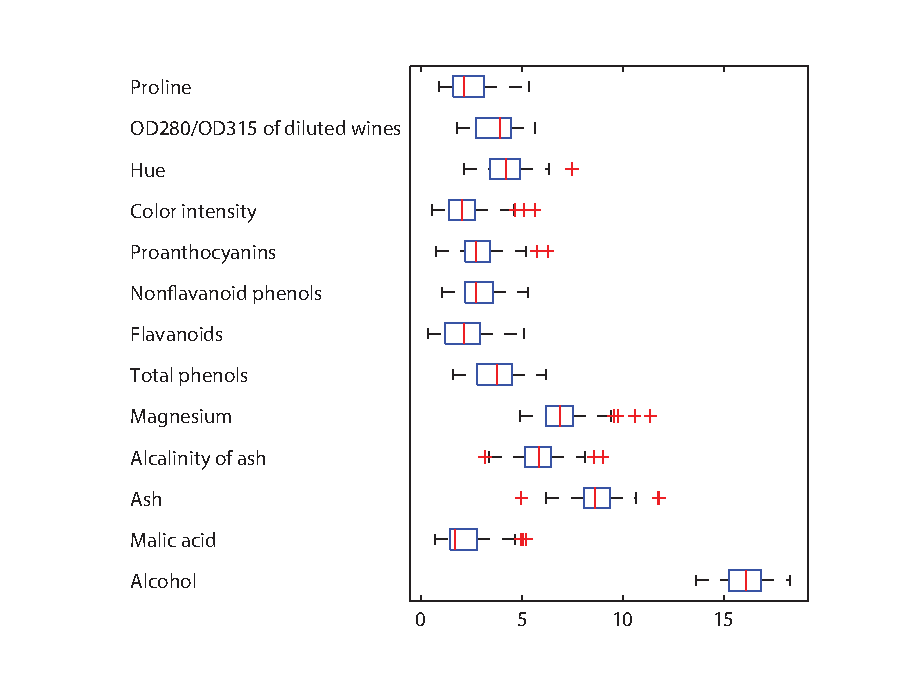
\includegraphics{img/boxplot.eps}
		\caption{Boxplots of all features of the dataset}
		\label{fig:boxes}
	\end{figure}

\begin{figure}
	\centering
	\newlength\figureheight 
	\newlength\figurewidth 
	\setlength\figureheight{7cm} 
	\setlength\figurewidth{9cm}
	% This file was created by matlab2tikz v0.4.3.
% Copyright (c) 2008--2013, Nico Schlömer <nico.schloemer@gmail.com>
% All rights reserved.
% 
% The latest updates can be retrieved from
%   http://www.mathworks.com/matlabcentral/fileexchange/22022-matlab2tikz
% where you can also make suggestions and rate matlab2tikz.
% 
\begin{tikzpicture}

\begin{axis}[%
width=\figurewidth,
height=\figureheight,
scale only axis,
xmin=-5,
xmax=5,
xlabel={1st Principal Component},
ymin=-4,
ymax=4,
ylabel={2nd Principal Component},
axis x line*=bottom,
axis y line*=left,
legend style={draw=black,fill=white,legend cell align=left}
]
\addplot [
color=red,
mark size=2.5pt,
only marks,
mark=*,
mark options={solid}
]
table[row sep=crcr]{
3.30742097428923 1.4394022531823\\
2.20324981342023 -0.332455071194179\\
2.50966069476186 1.0282507242942\\
3.74649719049799 2.74861839085854\\
1.0060704895977 0.867384035075406\\
3.04167372561128 2.11643091683108\\
2.44220051482514 1.17154534273535\\
2.0536437885938 1.60443714359377\\
2.50381134586223 0.915488474138317\\
2.74588238273254 0.787217029001901\\
3.46994837450078 1.29866984523335\\
1.74981687772954 0.610255770402337\\
2.10751728679335 0.673805614310881\\
3.44842921407716 1.12744947640952\\
4.30065228243313 2.09007971112926\\
2.29870383298749 1.6578750632565\\
2.16584568280965 2.32075875406352\\
1.89362947490782 1.626779927559\\
3.53202167238386 2.51125970683683\\
2.07865855822098 1.05815307067065\\
3.11561376238392 0.784683607297995\\
1.08351360638914 0.24106353999609\\
2.52809263376572 -0.0915822780973847\\
1.64036107937009 -0.514826665783717\\
1.75662065606153 -0.31625681015009\\
0.987294063457223 0.938021292616493\\
1.77028386961871 0.684244961307348\\
1.23194878453037 -0.0895544190842249\\
2.18225046758958 0.687629899180147\\
2.24976267059306 0.190923364970596\\
2.49318704413373 1.23734343744848\\
2.66987963717323 1.46773334635132\\
1.62399801279501 0.052556195849642\\
1.89733869731164 1.62846672543164\\
1.40642118110875 0.695971073676941\\
1.89847087353463 0.1762138728925\\
1.38096668895791 0.656787135916018\\
1.11905070261155 0.113788775806475\\
1.4979689099673 -0.767267636443276\\
2.52268490079999 1.79793023049862\\
2.5808152555232 0.777423286334352\\
0.666601590609367 0.169482849825774\\
3.06216897895342 1.15266742005172\\
0.460908968590187 0.329811772734117\\
2.09544094293404 -0.0708091767582304\\
1.13297020448577 1.77210848745488\\
2.71893118483658 1.18798353288002\\
2.81340300172213 0.644440709185732\\
2.00419725082142 1.24352163527515\\
2.69987527988475 1.74703921908322\\
3.20587408843523 0.166522255683714\\
2.85091772969851 0.743182375634174\\
3.49574328334839 1.6081973242466\\
2.21853316453292 1.86989325493805\\
2.14094846469849 1.01389147150761\\
2.46238339554064 1.32526988324217\\
2.73380617491011 1.43250785065951\\
2.16762630710584 1.20878998910284\\
3.13054924783241 1.72670827901314\\
};
\addlegendentry{1};

\addplot [
color=green,
mark size=2.5pt,
only marks,
mark=*,
mark options={solid}
]
table[row sep=crcr]{
-0.925969918827914 -3.06484061536441\\
-1.53814122596025 -1.37755758335536\\
-1.83108449370326 -0.827649423288587\\
0.0305207387428916 -1.25923399612215\\
2.04449433424567 -1.91961759362888\\
-0.607965828485849 -1.90269154043018\\
0.897695547224684 -0.761762632577595\\
2.242182263527 -1.87929122936635\\
0.182868177486559 -2.42031868594756\\
-0.810518651437925 -0.21989369316463\\
1.97006318680866 -1.39933586664535\\
-1.56779366172445 -0.882493727934894\\
1.65301884092157 -0.954021018576849\\
-0.723331955335034 -1.06065342459432\\
2.55501976881364 0.25946662641804\\
1.82741265809378 -1.28425546720206\\
-0.865551286816661 -2.43722606314141\\
0.368973574091478 -2.14784815309808\\
-1.45327752329742 -1.37946047650402\\
1.25937829459057 -0.768681172566499\\
0.375092281590871 -1.02415438665293\\
0.759920260189148 -3.36555996890649\\
1.03166775614799 -1.44662897140294\\
-0.493484694538252 -2.3745452194709\\
-2.53183508116183 -0.0871973839420364\\
0.83297043568931 -1.46952519705299\\
0.78568828256836 -2.02092573332855\\
-0.804562581410654 -2.22754674860494\\
-0.556472881611739 -2.36631035112901\\
-1.11197429578471 -1.79717756926931\\
-0.554159612143509 -2.65006452118737\\
-1.34548981702795 -2.1120436479411\\
-1.56008180204935 -1.84700434401334\\
-1.92711943780747 -1.55510868180387\\
0.744565611690007 -2.30642555931631\\
0.954762094435214 -2.21727377126558\\
2.53670943110962 0.168797864267749\\
-0.542422480010212 -0.367888775760008\\
1.02814946405103 -2.55835254302044\\
2.24557492458675 -1.42871115751728\\
1.4062491551155 -2.16009839085986\\
0.795475850715722 -2.37026257660731\\
-0.547985924074936 -2.28667819827848\\
-0.160720367067457 -1.16120769391348\\
-0.657938974740039 -2.67242260231914\\
0.391250736777433 -2.09282809170154\\
-1.76751313537439 -1.71245783120106\\
-0.365237067386073 -2.16325102611279\\
-1.61611370982472 -1.35177020638497\\
0.0823036148660643 -2.29974727647888\\
1.57383546981447 -1.45792166802079\\
1.41657326452753 -1.41421730023\\
-0.277918778105264 -1.92513750663662\\
-1.29947929100858 -0.761025551842137\\
-0.455786147590487 -2.26303186608984\\
-0.492795729390357 -1.93359062222765\\
0.480718360927135 -3.86089273302546\\
-0.252177515125454 -2.81355567156815\\
-0.10692601227162 -1.92349609077043\\
-2.426168671686 -1.25360477177194\\
-0.549539354559022 -2.21591073234407\\
0.737541412692771 -1.40499334962045\\
1.33256273375419 0.252624308290619\\
-1.17377591515635 -0.66209913753691\\
-0.461034485027037 -0.616548968783821\\
0.975721685495425 -1.44150418845279\\
-0.0965374058712812 -2.10406268463188\\
0.0383788837206458 -1.26319877689754\\
-1.592665782037 -1.20474513258868\\
-0.478215926305124 -1.93338680807016\\
-1.78779033090865 -1.14705240716191\\
};
\addlegendentry{2};

\addplot [
color=blue,
mark size=2.5pt,
only marks,
mark=*,
mark options={solid}
]
table[row sep=crcr]{
-1.32336859204859 0.169909936494653\\
-2.37779336481857 0.373528925222153\\
-2.92867865089463 0.263119601227974\\
-2.14077227196925 0.36721907092618\\
-2.36320317558219 -0.458341881749459\\
-3.05522315061054 0.352418704556715\\
-3.90473898331631 0.154147687302041\\
-3.92539033533296 0.657831569442927\\
-3.08557208893704 0.34786148374549\\
-2.36779236968985 0.291159026862504\\
-2.77099629938406 0.285998106522041\\
-2.28012931339022 0.371460000571083\\
-2.97723506437817 0.487841765231787\\
-2.36851340595321 0.480976938981241\\
-2.20364929520704 1.15678934015719\\
-2.61823527696862 0.561576623901966\\
-4.2685975768988 0.647843475272684\\
-3.57256359852983 1.26912270677122\\
-2.79916760396144 1.56611596172983\\
-2.89150275052853 2.03531562664122\\
-2.31420887085633 2.34973774716454\\
-2.54265841277236 2.03952982198261\\
-1.80744270572725 1.52334876209868\\
-2.75238050659446 2.13291564838871\\
-2.72945104659534 0.408733283306981\\
-3.59472856998581 1.79731420974145\\
-2.88169707501281 1.91980307887748\\
-3.38261412804098 1.30818615222258\\
-1.0452334187292 3.50520193691751\\
-1.60538368798997 2.39986841857009\\
-3.13428951191097 0.736084637687935\\
-2.23385545791818 1.17215876880337\\
-2.8396634261414 0.554479844736746\\
-2.59019044004634 0.696002198467208\\
-2.94100315593216 1.5509339655631\\
-3.52010247940368 0.88004429678245\\
-2.39934228363786 2.58506401945767\\
-2.92084537245454 1.27086199861469\\
-2.17527658443826 2.07169331434286\\
-2.37423036799742 2.58138565306433\\
-3.20258311215209 -0.250542354489897\\
-3.66757293755117 0.845363176010537\\
-2.45862032495413 2.1876272694784\\
-3.36104304608341 2.21005484019807\\
-2.59463669227798 1.75228636129724\\
-2.67030684549029 2.75313287400681\\
-2.38030254326328 2.29088436964069\\
-3.1997321036619 2.76113074733832\\
};
\addlegendentry{3};

\end{axis}
\end{tikzpicture}%
	\caption{Scatterplot of the dataset with principal components}
	\label{fig:scatter}
\end{figure}

\begin{figure}
	\centering
	\setlength\figureheight{7cm} 
	\setlength\figurewidth{7cm}
	% This file was created by matlab2tikz v0.4.3.
% Copyright (c) 2008--2013, Nico Schlömer <nico.schloemer@gmail.com>
% All rights reserved.
% 
% The latest updates can be retrieved from
%   http://www.mathworks.com/matlabcentral/fileexchange/22022-matlab2tikz
% where you can also make suggestions and rate matlab2tikz.
% 
\begin{tikzpicture}

\begin{axis}[%
width=\figurewidth,
height=\figureheight,
unbounded coords=jump,
view={-47.5}{32},
scale only axis,
xmin=-0.688846290956282,
xmax=0.688846290956282,
xlabel={Component 1},
xmajorgrids,
ymin=-0.688846290956282,
ymax=0.688846290956282,
ylabel={Component 2},
ymajorgrids,
zmin=-0.688846290956282,
zmax=0.688846290956282,
zlabel={Component 3},
zmajorgrids,
axis x line*=bottom,
axis y line*=left,
axis z line*=left
]
\addplot3 [
color=blue,
solid]
table[row sep=crcr] {
0 0 0\\
0.144329395406011 0.483651547817214 -0.207382624116357\\
};
\addplot3 [
color=blue,
solid]
table[row sep=crcr] {
0 0 0\\
-0.245187580257221 0.224930934627845 0.0890128856596569\\
};
\addplot3 [
color=blue,
solid]
table[row sep=crcr] {
0 0 0\\
-0.00205106144437084 0.316068814025315 0.626223900869347\\
};
\addplot3 [
color=blue,
solid]
table[row sep=crcr] {
0 0 0\\
-0.239320405487535 -0.0105905022881914 0.612080349945782\\
};
\addplot3 [
color=blue,
solid]
table[row sep=crcr] {
0 0 0\\
0.141992041952987 0.299634003237862 0.130756934850279\\
};
\addplot3 [
color=blue,
solid]
table[row sep=crcr] {
0 0 0\\
0.39466084506663 0.0650395118192793 0.146178963484672\\
};
\addplot3 [
color=blue,
solid]
table[row sep=crcr] {
0 0 0\\
0.422934296710059 -0.00335981210030797 0.150681899899448\\
};
\addplot3 [
color=blue,
solid]
table[row sep=crcr] {
0 0 0\\
-0.298533102954715 0.028779488112987 0.17036816235965\\
};
\addplot3 [
color=blue,
solid]
table[row sep=crcr] {
0 0 0\\
0.313429488307689 0.0393017222897325 0.149454309462026\\
};
\addplot3 [
color=blue,
solid]
table[row sep=crcr] {
0 0 0\\
-0.0886167047247227 0.529995672070044 -0.137306212490242\\
};
\addplot3 [
color=blue,
solid]
table[row sep=crcr] {
0 0 0\\
0.296714563586381 -0.279235147924283 0.0852219225068911\\
};
\addplot3 [
color=blue,
solid]
table[row sep=crcr] {
0 0 0\\
0.376167410738713 -0.164496192835785 0.166004588087527\\
};
\addplot3 [
color=blue,
solid]
table[row sep=crcr] {
0 0 0\\
0.286752226896805 0.364902831798083 -0.126745917347702\\
};
\addplot3 [
color=blue,
only marks,
mark=*,
mark options={solid}]
table[row sep=crcr] {
0.144329395406011 0.483651547817214 -0.207382624116357\\
NaN NaN NaN\\
};
\addplot3 [
color=blue,
only marks,
mark=*,
mark options={solid}]
table[row sep=crcr] {
-0.245187580257221 0.224930934627845 0.0890128856596569\\
NaN NaN NaN\\
};
\addplot3 [
color=blue,
only marks,
mark=*,
mark options={solid}]
table[row sep=crcr] {
-0.00205106144437084 0.316068814025315 0.626223900869347\\
NaN NaN NaN\\
};
\addplot3 [
color=blue,
only marks,
mark=*,
mark options={solid}]
table[row sep=crcr] {
-0.239320405487535 -0.0105905022881914 0.612080349945782\\
NaN NaN NaN\\
};
\addplot3 [
color=blue,
only marks,
mark=*,
mark options={solid}]
table[row sep=crcr] {
0.141992041952987 0.299634003237862 0.130756934850279\\
NaN NaN NaN\\
};
\addplot3 [
color=blue,
only marks,
mark=*,
mark options={solid}]
table[row sep=crcr] {
0.39466084506663 0.0650395118192793 0.146178963484672\\
NaN NaN NaN\\
};
\addplot3 [
color=blue,
only marks,
mark=*,
mark options={solid}]
table[row sep=crcr] {
0.422934296710059 -0.00335981210030797 0.150681899899448\\
NaN NaN NaN\\
};
\addplot3 [
color=blue,
only marks,
mark=*,
mark options={solid}]
table[row sep=crcr] {
-0.298533102954715 0.028779488112987 0.17036816235965\\
NaN NaN NaN\\
};
\addplot3 [
color=blue,
only marks,
mark=*,
mark options={solid}]
table[row sep=crcr] {
0.313429488307689 0.0393017222897325 0.149454309462026\\
NaN NaN NaN\\
};
\addplot3 [
color=blue,
only marks,
mark=*,
mark options={solid}]
table[row sep=crcr] {
-0.0886167047247227 0.529995672070044 -0.137306212490242\\
NaN NaN NaN\\
};
\addplot3 [
color=blue,
only marks,
mark=*,
mark options={solid}]
table[row sep=crcr] {
0.296714563586381 -0.279235147924283 0.0852219225068911\\
NaN NaN NaN\\
};
\addplot3 [
color=blue,
only marks,
mark=*,
mark options={solid}]
table[row sep=crcr] {
0.376167410738713 -0.164496192835785 0.166004588087527\\
NaN NaN NaN\\
};
\addplot3 [
color=blue,
only marks,
mark=*,
mark options={solid}]
table[row sep=crcr] {
0.286752226896805 0.364902831798083 -0.126745917347702\\
NaN NaN NaN\\
};
\node[right, inner sep=0mm, text=black]
at (axis cs:0.152329395406011,0.492651547817214,-0.187382624116357) {Alcohol};
\node[right, inner sep=0mm, text=black]
at (axis cs:-0.237187580257221,0.233930934627845,0.109012885659657) {Malic acid};
\node[right, inner sep=0mm, text=black]
at (axis cs:0.00594893855562916,0.325068814025315,0.646223900869347) {Ash};
\node[right, inner sep=0mm, text=black]
at (axis cs:-0.231320405487535,-0.00159050228819139,0.632080349945782) {Alcalinity of ash};
\node[right, inner sep=0mm, text=black]
at (axis cs:0.149992041952987,0.308634003237862,0.150756934850279) {Magnesium};
\node[right, inner sep=0mm, text=black]
at (axis cs:0.40266084506663,0.0740395118192793,0.166178963484672) {Total phenols};
\node[right, inner sep=0mm, text=black]
at (axis cs:0.430934296710059,0.00564018789969203,0.170681899899448) {Flavanoids};
\node[right, inner sep=0mm, text=black]
at (axis cs:-0.290533102954715,0.037779488112987,0.19036816235965) {Nonflavanoid phenols};
\node[right, inner sep=0mm, text=black]
at (axis cs:0.321429488307689,0.0483017222897325,0.169454309462026) {Proanthocyanins};
\node[right, inner sep=0mm, text=black]
at (axis cs:-0.0806167047247227,0.538995672070044,-0.117306212490242) {Color intensity};
\node[right, inner sep=0mm, text=black]
at (axis cs:0.304714563586381,-0.270235147924282,0.105221922506891) {Hue};
\node[right, inner sep=0mm, text=black]
at (axis cs:0.384167410738713,-0.155496192835785,0.186004588087527) {OD280/OD315 of diluted wines};
\node[right, inner sep=0mm, text=black]
at (axis cs:0.294752226896805,0.373902831798083,-0.106745917347702) {Proline};
\addplot3 [
color=black,
solid]
table[row sep=crcr] {
-0.688846290956282 0 0\\
0.688846290956282 0 0\\
NaN NaN NaN\\
0 -0.688846290956282 0\\
0 0.688846290956282 0\\
NaN NaN NaN\\
0 0 -0.688846290956282\\
0 0 0.688846290956282\\
};
\addplot3 [
color=red,
only marks,
mark=*,
mark options={solid}]
table[row sep=crcr] {
0.435253888717558 0.189424156464101 -0.0217497689048848\\
NaN NaN NaN\\
};
\addplot3 [
color=red,
only marks,
mark=*,
mark options={solid}]
table[row sep=crcr] {
0.289945869171817 -0.0437508148149286 -0.265929972496525\\
NaN NaN NaN\\
};
\addplot3 [
color=red,
only marks,
mark=*,
mark options={solid}]
table[row sep=crcr] {
0.33026928995377 0.135316952333796 0.128974310201002\\
NaN NaN NaN\\
};
\addplot3 [
color=red,
only marks,
mark=*,
mark options={solid}]
table[row sep=crcr] {
0.493035958805967 0.36171592685714 -0.0231214790677726\\
NaN NaN NaN\\
};
\addplot3 [
color=red,
only marks,
mark=*,
mark options={solid}]
table[row sep=crcr] {
0.132398051631599 0.114147027914773 0.265960266110926\\
NaN NaN NaN\\
};
\addplot3 [
color=red,
only marks,
mark=*,
mark options={solid}]
table[row sep=crcr] {
0.400281768657176 0.27852057355679 -0.0825949843004749\\
NaN NaN NaN\\
};
\addplot3 [
color=red,
only marks,
mark=*,
mark options={solid}]
table[row sep=crcr] {
0.321391585579486 0.154174406644467 -0.128223184347523\\
NaN NaN NaN\\
};
\addplot3 [
color=red,
only marks,
mark=*,
mark options={solid}]
table[row sep=crcr] {
0.270257838955079 0.211142612742895 0.0191964250726911\\
NaN NaN NaN\\
};
\addplot3 [
color=red,
only marks,
mark=*,
mark options={solid}]
table[row sep=crcr] {
0.329499520434007 0.120477532658339 -0.2324024925421\\
NaN NaN NaN\\
};
\addplot3 [
color=red,
only marks,
mark=*,
mark options={solid}]
table[row sep=crcr] {
0.361355870430801 0.103597115638233 -0.129161812728175\\
NaN NaN NaN\\
};
\addplot3 [
color=red,
only marks,
mark=*,
mark options={solid}]
table[row sep=crcr] {
0.45664236134174 0.170903886953646 -0.0554751192754845\\
NaN NaN NaN\\
};
\addplot3 [
color=red,
only marks,
mark=*,
mark options={solid}]
table[row sep=crcr] {
0.230274466569552 0.0803091590833936 -0.1562777697075\\
NaN NaN NaN\\
};
\addplot3 [
color=red,
only marks,
mark=*,
mark options={solid}]
table[row sep=crcr] {
0.277347547151421 0.0886722664421511 -0.113524425603439\\
NaN NaN NaN\\
};
\addplot3 [
color=red,
only marks,
mark=*,
mark options={solid}]
table[row sep=crcr] {
0.453810457471888 0.148371426786781 -0.158035980153369\\
NaN NaN NaN\\
};
\addplot3 [
color=red,
only marks,
mark=*,
mark options={solid}]
table[row sep=crcr] {
0.565962314595689 0.275052776489748 -0.16586200520026\\
NaN NaN NaN\\
};
\addplot3 [
color=red,
only marks,
mark=*,
mark options={solid}]
table[row sep=crcr] {
0.302507539891493 0.218174999160889 0.0285951421043095\\
NaN NaN NaN\\
};
\addplot3 [
color=red,
only marks,
mark=*,
mark options={solid}]
table[row sep=crcr] {
0.285023516248221 0.305409949423972 0.10914707767606\\
NaN NaN NaN\\
};
\addplot3 [
color=red,
only marks,
mark=*,
mark options={solid}]
table[row sep=crcr] {
0.249200086457377 0.214082904795597 0.104315741193124\\
NaN NaN NaN\\
};
\addplot3 [
color=red,
only marks,
mark=*,
mark options={solid}]
table[row sep=crcr] {
0.464811156454052 0.330479718631928 -0.0637062339729053\\
NaN NaN NaN\\
};
\addplot3 [
color=red,
only marks,
mark=*,
mark options={solid}]
table[row sep=crcr] {
0.27354976213034 0.139252076602314 -0.0216195416930695\\
NaN NaN NaN\\
};
\addplot3 [
color=red,
only marks,
mark=*,
mark options={solid}]
table[row sep=crcr] {
0.410012216878732 0.103263719418956 -0.0478837666154519\\
NaN NaN NaN\\
};
\addplot3 [
color=red,
only marks,
mark=*,
mark options={solid}]
table[row sep=crcr] {
0.142589502311723 0.0317237642341151 0.122956532733079\\
NaN NaN NaN\\
};
\addplot3 [
color=red,
only marks,
mark=*,
mark options={solid}]
table[row sep=crcr] {
0.332694918015754 -0.0120521527163822 -0.0409346106132568\\
NaN NaN NaN\\
};
\addplot3 [
color=red,
only marks,
mark=*,
mark options={solid}]
table[row sep=crcr] {
0.2158701732398 -0.0677507671505325 0.0188818969315744\\
NaN NaN NaN\\
};
\addplot3 [
color=red,
only marks,
mark=*,
mark options={solid}]
table[row sep=crcr] {
0.231169838220148 -0.0416191369412291 0.116831294252099\\
NaN NaN NaN\\
};
\addplot3 [
color=red,
only marks,
mark=*,
mark options={solid}]
table[row sep=crcr] {
0.129927089344852 0.12344283309715 0.501413932838788\\
NaN NaN NaN\\
};
\addplot3 [
color=red,
only marks,
mark=*,
mark options={solid}]
table[row sep=crcr] {
0.232967905922861 0.0900460759484722 -0.0113776075485245\\
NaN NaN NaN\\
};
\addplot3 [
color=red,
only marks,
mark=*,
mark options={solid}]
table[row sep=crcr] {
0.162123450064576 -0.0117852881327353 -0.182001045177111\\
NaN NaN NaN\\
};
\addplot3 [
color=red,
only marks,
mark=*,
mark options={solid}]
table[row sep=crcr] {
0.287182372476245 0.0904915309974835 0.183007615685639\\
NaN NaN NaN\\
};
\addplot3 [
color=red,
only marks,
mark=*,
mark options={solid}]
table[row sep=crcr] {
0.296066923043464 0.0251253583068155 -0.143388318053467\\
NaN NaN NaN\\
};
\addplot3 [
color=red,
only marks,
mark=*,
mark options={solid}]
table[row sep=crcr] {
0.32810137103658 0.162833381965941 0.181885735544337\\
NaN NaN NaN\\
};
\addplot3 [
color=red,
only marks,
mark=*,
mark options={solid}]
table[row sep=crcr] {
0.351353971423974 0.193152505098669 -0.0436023739904383\\
NaN NaN NaN\\
};
\addplot3 [
color=red,
only marks,
mark=*,
mark options={solid}]
table[row sep=crcr] {
0.213716807093333 0.00691635228704872 -0.0219321328095321\\
NaN NaN NaN\\
};
\addplot3 [
color=red,
only marks,
mark=*,
mark options={solid}]
table[row sep=crcr] {
0.249688217084814 0.214304886012761 0.153811163138519\\
NaN NaN NaN\\
};
\addplot3 [
color=red,
only marks,
mark=*,
mark options={solid}]
table[row sep=crcr] {
0.185083874417854 0.0915892227229772 0.0629561969264579\\
NaN NaN NaN\\
};
\addplot3 [
color=red,
only marks,
mark=*,
mark options={solid}]
table[row sep=crcr] {
0.249837210547575 0.023189601208514 0.0591626309771811\\
NaN NaN NaN\\
};
\addplot3 [
color=red,
only marks,
mark=*,
mark options={solid}]
table[row sep=crcr] {
0.181734084118974 0.0864326486375227 0.0601604360264782\\
NaN NaN NaN\\
};
\addplot3 [
color=red,
only marks,
mark=*,
mark options={solid}]
table[row sep=crcr] {
0.147266155040474 0.0149745096095069 -0.00513200877005377\\
NaN NaN NaN\\
};
\addplot3 [
color=red,
only marks,
mark=*,
mark options={solid}]
table[row sep=crcr] {
0.19713148048273 -0.100971791932484 -0.1871558253679\\
NaN NaN NaN\\
};
\addplot3 [
color=red,
only marks,
mark=*,
mark options={solid}]
table[row sep=crcr] {
0.331983264790846 0.236606144349542 -0.0450315444790372\\
NaN NaN NaN\\
};
\addplot3 [
color=red,
only marks,
mark=*,
mark options={solid}]
table[row sep=crcr] {
0.339633171815834 0.102308267132317 -0.015547679271381\\
NaN NaN NaN\\
};
\addplot3 [
color=red,
only marks,
mark=*,
mark options={solid}]
table[row sep=crcr] {
0.0877242228290543 0.0223038040911786 -0.102799882964868\\
NaN NaN NaN\\
};
\addplot3 [
color=red,
only marks,
mark=*,
mark options={solid}]
table[row sep=crcr] {
0.402978927194526 0.15169008749585 -0.0410429302553767\\
NaN NaN NaN\\
};
\addplot3 [
color=red,
only marks,
mark=*,
mark options={solid}]
table[row sep=crcr] {
0.060655242402818 0.0434029589046206 -0.0264395589074698\\
NaN NaN NaN\\
};
\addplot3 [
color=red,
only marks,
mark=*,
mark options={solid}]
table[row sep=crcr] {
0.275758310199998 -0.00931842961041025 -0.0860664621712038\\
NaN NaN NaN\\
};
\addplot3 [
color=red,
only marks,
mark=*,
mark options={solid}]
table[row sep=crcr] {
0.149097950075597 0.233208024134238 0.00376702496997846\\
NaN NaN NaN\\
};
\addplot3 [
color=red,
only marks,
mark=*,
mark options={solid}]
table[row sep=crcr] {
0.357809114882896 0.156337658991103 -0.0708339046982559\\
NaN NaN NaN\\
};
\addplot3 [
color=red,
only marks,
mark=*,
mark options={solid}]
table[row sep=crcr] {
0.370241528534893 0.0848078690016984 -0.15164198604664\\
NaN NaN NaN\\
};
\addplot3 [
color=red,
only marks,
mark=*,
mark options={solid}]
table[row sep=crcr] {
0.26375071512163 0.163646427734903 -0.00751863268086083\\
NaN NaN NaN\\
};
\addplot3 [
color=red,
only marks,
mark=*,
mark options={solid}]
table[row sep=crcr] {
0.355301373413701 0.229908928968883 -0.0843951554876159\\
NaN NaN NaN\\
};
\addplot3 [
color=red,
only marks,
mark=*,
mark options={solid}]
table[row sep=crcr] {
0.421890401789618 0.0219141923292459 -0.258989835828611\\
NaN NaN NaN\\
};
\addplot3 [
color=red,
only marks,
mark=*,
mark options={solid}]
table[row sep=crcr] {
0.375178435981157 0.0978021913556504 0.00061933554442136\\
NaN NaN NaN\\
};
\addplot3 [
color=red,
only marks,
mark=*,
mark options={solid}]
table[row sep=crcr] {
0.460036950198833 0.211637449434125 -0.0683407202392019\\
NaN NaN NaN\\
};
\addplot3 [
color=red,
only marks,
mark=*,
mark options={solid}]
table[row sep=crcr] {
0.291957145648608 0.246076419368847 0.0445587869416827\\
NaN NaN NaN\\
};
\addplot3 [
color=red,
only marks,
mark=*,
mark options={solid}]
table[row sep=crcr] {
0.281747062756098 0.133427286439124 -0.125686248443061\\
NaN NaN NaN\\
};
\addplot3 [
color=red,
only marks,
mark=*,
mark options={solid}]
table[row sep=crcr] {
0.324047636135261 0.174404430148291 0.0673778829642964\\
NaN NaN NaN\\
};
\addplot3 [
color=red,
only marks,
mark=*,
mark options={solid}]
table[row sep=crcr] {
0.359766651381719 0.188516858744289 -0.0803742705783327\\
NaN NaN NaN\\
};
\addplot3 [
color=red,
only marks,
mark=*,
mark options={solid}]
table[row sep=crcr] {
0.285257844945804 0.15907577157242 0.0343530738941157\\
NaN NaN NaN\\
};
\addplot3 [
color=red,
only marks,
mark=*,
mark options={solid}]
table[row sep=crcr] {
0.411977714519302 0.227233393923428 -0.037487061204588\\
NaN NaN NaN\\
};
\addplot3 [
color=red,
only marks,
mark=*,
mark options={solid}]
table[row sep=crcr] {
-0.121856882186563 -0.403330512355944 -0.601693359591747\\
NaN NaN NaN\\
};
\addplot3 [
color=red,
only marks,
mark=*,
mark options={solid}]
table[row sep=crcr] {
-0.202418124333223 -0.181285448616541 -0.114783789208872\\
NaN NaN NaN\\
};
\addplot3 [
color=red,
only marks,
mark=*,
mark options={solid}]
table[row sep=crcr] {
-0.240969218206654 -0.108917985578965 -0.210714690456848\\
NaN NaN NaN\\
};
\addplot3 [
color=red,
only marks,
mark=*,
mark options={solid}]
table[row sep=crcr] {
0.00401650419696906 -0.165714161541018 -0.234166076852467\\
NaN NaN NaN\\
};
\addplot3 [
color=red,
only marks,
mark=*,
mark options={solid}]
table[row sep=crcr] {
0.269053778263796 -0.252620101575417 -0.000966997274800615\\
NaN NaN NaN\\
};
\addplot3 [
color=red,
only marks,
mark=*,
mark options={solid}]
table[row sep=crcr] {
-0.0800078046045301 -0.250392646850831 0.0891514621016737\\
NaN NaN NaN\\
};
\addplot3 [
color=red,
only marks,
mark=*,
mark options={solid}]
table[row sep=crcr] {
0.118135998063551 -0.100247337936888 0.0752416296873743\\
NaN NaN NaN\\
};
\addplot3 [
color=red,
only marks,
mark=*,
mark options={solid}]
table[row sep=crcr] {
0.29506934768816 -0.247313185098938 -0.266636354453083\\
NaN NaN NaN\\
};
\addplot3 [
color=red,
only marks,
mark=*,
mark options={solid}]
table[row sep=crcr] {
0.024065302237742 -0.318511954838417 -0.140381638958667\\
NaN NaN NaN\\
};
\addplot3 [
color=red,
only marks,
mark=*,
mark options={solid}]
table[row sep=crcr] {
-0.106663590047614 -0.0289378297466166 -0.0927796103142226\\
NaN NaN NaN\\
};
\addplot3 [
color=red,
only marks,
mark=*,
mark options={solid}]
table[row sep=crcr] {
0.259258700281432 -0.184151452843173 -0.162497748682066\\
NaN NaN NaN\\
};
\addplot3 [
color=red,
only marks,
mark=*,
mark options={solid}]
table[row sep=crcr] {
-0.206320360570051 -0.116135451107811 -0.0825427713247056\\
NaN NaN NaN\\
};
\addplot3 [
color=red,
only marks,
mark=*,
mark options={solid}]
table[row sep=crcr] {
0.217535924282853 -0.125548383916594 0.256235672030745\\
NaN NaN NaN\\
};
\addplot3 [
color=red,
only marks,
mark=*,
mark options={solid}]
table[row sep=crcr] {
-0.0951898923181095 -0.139581121128822 0.0105419179413322\\
NaN NaN NaN\\
};
\addplot3 [
color=red,
only marks,
mark=*,
mark options={solid}]
table[row sep=crcr] {
0.336238506912583 0.034145595319975 0.442818341589296\\
NaN NaN NaN\\
};
\addplot3 [
color=red,
only marks,
mark=*,
mark options={solid}]
table[row sep=crcr] {
0.2404860076507 -0.169006966621963 0.0601396292156322\\
NaN NaN NaN\\
};
\addplot3 [
color=red,
only marks,
mark=*,
mark options={solid}]
table[row sep=crcr] {
-0.11390583974645 -0.320736951816075 -0.205154648034883\\
NaN NaN NaN\\
};
\addplot3 [
color=red,
only marks,
mark=*,
mark options={solid}]
table[row sep=crcr] {
0.0485566198575143 -0.282655056092962 -0.321430518429271\\
NaN NaN NaN\\
};
\addplot3 [
color=red,
only marks,
mark=*,
mark options={solid}]
table[row sep=crcr] {
-0.191250130635989 -0.181535867794871 -0.0298292572375188\\
NaN NaN NaN\\
};
\addplot3 [
color=red,
only marks,
mark=*,
mark options={solid}]
table[row sep=crcr] {
0.165733151101163 -0.101157812127451 -0.155404597898647\\
NaN NaN NaN\\
};
\addplot3 [
color=red,
only marks,
mark=*,
mark options={solid}]
table[row sep=crcr] {
0.0493618367481789 -0.134777877658476 0.235486015408775\\
NaN NaN NaN\\
};
\addplot3 [
color=red,
only marks,
mark=*,
mark options={solid}]
table[row sep=crcr] {
0.100004883240987 -0.442904932745519 -0.0469104375283894\\
NaN NaN NaN\\
};
\addplot3 [
color=red,
only marks,
mark=*,
mark options={solid}]
table[row sep=crcr] {
0.135766630924395 -0.190375186657309 -0.0476376715844882\\
NaN NaN NaN\\
};
\addplot3 [
color=red,
only marks,
mark=*,
mark options={solid}]
table[row sep=crcr] {
-0.0649421812312626 -0.312488204176217 0.17528823982339\\
NaN NaN NaN\\
};
\addplot3 [
color=red,
only marks,
mark=*,
mark options={solid}]
table[row sep=crcr] {
-0.333187421024939 -0.0114751042403743 0.0622355355042934\\
NaN NaN NaN\\
};
\addplot3 [
color=red,
only marks,
mark=*,
mark options={solid}]
table[row sep=crcr] {
0.109618226448613 -0.193388311182009 0.0800619691788866\\
NaN NaN NaN\\
};
\addplot3 [
color=red,
only marks,
mark=*,
mark options={solid}]
table[row sep=crcr] {
0.10339593386088 -0.265952169705178 -0.0334270973016174\\
NaN NaN NaN\\
};
\addplot3 [
color=red,
only marks,
mark=*,
mark options={solid}]
table[row sep=crcr] {
-0.105879776114947 -0.293143325922946 0.101421092567345\\
NaN NaN NaN\\
};
\addplot3 [
color=red,
only marks,
mark=*,
mark options={solid}]
table[row sep=crcr] {
-0.0732313750109858 -0.311404502253557 0.302825534419486\\
NaN NaN NaN\\
};
\addplot3 [
color=red,
only marks,
mark=*,
mark options={solid}]
table[row sep=crcr] {
-0.14633490570346 -0.236507094748813 0.125881851268128\\
NaN NaN NaN\\
};
\addplot3 [
color=red,
only marks,
mark=*,
mark options={solid}]
table[row sep=crcr] {
-0.0729269506454376 -0.348746318405117 0.111430072737547\\
NaN NaN NaN\\
};
\addplot3 [
color=red,
only marks,
mark=*,
mark options={solid}]
table[row sep=crcr] {
-0.177065356857738 -0.277943212567651 -0.00625336636066508\\
NaN NaN NaN\\
};
\addplot3 [
color=red,
only marks,
mark=*,
mark options={solid}]
table[row sep=crcr] {
-0.205305486159166 -0.243064257456004 0.102498644550376\\
NaN NaN NaN\\
};
\addplot3 [
color=red,
only marks,
mark=*,
mark options={solid}]
table[row sep=crcr] {
-0.253607338119137 -0.204651027611939 -0.0117154263736676\\
NaN NaN NaN\\
};
\addplot3 [
color=red,
only marks,
mark=*,
mark options={solid}]
table[row sep=crcr] {
0.0979842240865897 -0.303523712745919 0.0150493112475758\\
NaN NaN NaN\\
};
\addplot3 [
color=red,
only marks,
mark=*,
mark options={solid}]
table[row sep=crcr] {
0.125645908892004 -0.291791410527106 0.0186928850523019\\
NaN NaN NaN\\
};
\addplot3 [
color=red,
only marks,
mark=*,
mark options={solid}]
table[row sep=crcr] {
0.333828881481965 0.0222136605533092 0.103499916538069\\
NaN NaN NaN\\
};
\addplot3 [
color=red,
only marks,
mark=*,
mark options={solid}]
table[row sep=crcr] {
-0.0713823536790635 -0.0484138612864352 0.171765102813637\\
NaN NaN NaN\\
};
\addplot3 [
color=red,
only marks,
mark=*,
mark options={solid}]
table[row sep=crcr] {
0.135303626568811 -0.336677097265914 -0.142565894934677\\
NaN NaN NaN\\
};
\addplot3 [
color=red,
only marks,
mark=*,
mark options={solid}]
table[row sep=crcr] {
0.295515819102242 -0.188017217039387 -0.030209997374187\\
NaN NaN NaN\\
};
\addplot3 [
color=red,
only marks,
mark=*,
mark options={solid}]
table[row sep=crcr] {
0.185061235938174 -0.28426717733939 0.0982769262720048\\
NaN NaN NaN\\
};
\addplot3 [
color=red,
only marks,
mark=*,
mark options={solid}]
table[row sep=crcr] {
0.104683969805002 -0.311924611886377 -0.205781837655946\\
NaN NaN NaN\\
};
\addplot3 [
color=red,
only marks,
mark=*,
mark options={solid}]
table[row sep=crcr] {
-0.0721144983569432 -0.300924976222676 -0.196703781893016\\
NaN NaN NaN\\
};
\addplot3 [
color=red,
only marks,
mark=*,
mark options={solid}]
table[row sep=crcr] {
-0.0211506685438667 -0.152813980534547 0.131716265677192\\
NaN NaN NaN\\
};
\addplot3 [
color=red,
only marks,
mark=*,
mark options={solid}]
table[row sep=crcr] {
-0.0865842296824603 -0.351688623552395 -0.10037979981517\\
NaN NaN NaN\\
};
\addplot3 [
color=red,
only marks,
mark=*,
mark options={solid}]
table[row sep=crcr] {
0.0514882762036615 -0.275414461119875 -0.0619204041338308\\
NaN NaN NaN\\
};
\addplot3 [
color=red,
only marks,
mark=*,
mark options={solid}]
table[row sep=crcr] {
-0.23260327956782 -0.225358046674199 0.124278215418111\\
NaN NaN NaN\\
};
\addplot3 [
color=red,
only marks,
mark=*,
mark options={solid}]
table[row sep=crcr] {
-0.0480648986383562 -0.284682061554073 -0.063163697475872\\
NaN NaN NaN\\
};
\addplot3 [
color=red,
only marks,
mark=*,
mark options={solid}]
table[row sep=crcr] {
-0.212679239286173 -0.177891850948316 0.037683588188994\\
NaN NaN NaN\\
};
\addplot3 [
color=red,
only marks,
mark=*,
mark options={solid}]
table[row sep=crcr] {
0.0108310882419995 -0.302644856199522 -0.0608344817747948\\
NaN NaN NaN\\
};
\addplot3 [
color=red,
only marks,
mark=*,
mark options={solid}]
table[row sep=crcr] {
0.207115457561487 -0.191861296274208 0.233541157052099\\
NaN NaN NaN\\
};
\addplot3 [
color=red,
only marks,
mark=*,
mark options={solid}]
table[row sep=crcr] {
0.186419880272856 -0.186109837302775 0.018277027675955\\
NaN NaN NaN\\
};
\addplot3 [
color=red,
only marks,
mark=*,
mark options={solid}]
table[row sep=crcr] {
-0.0365738833545202 -0.253346517601886 0.0103238579200052\\
NaN NaN NaN\\
};
\addplot3 [
color=red,
only marks,
mark=*,
mark options={solid}]
table[row sep=crcr] {
-0.171010409354064 -0.100150338716377 0.262405048293118\\
NaN NaN NaN\\
};
\addplot3 [
color=red,
only marks,
mark=*,
mark options={solid}]
table[row sep=crcr] {
-0.0599810833590625 -0.297813138292452 0.139278450220296\\
NaN NaN NaN\\
};
\addplot3 [
color=red,
only marks,
mark=*,
mark options={solid}]
table[row sep=crcr] {
-0.0648515139826289 -0.254458940683608 0.173739067855504\\
NaN NaN NaN\\
};
\addplot3 [
color=red,
only marks,
mark=*,
mark options={solid}]
table[row sep=crcr] {
0.0632621421941702 -0.508090318418515 0.176407366908048\\
NaN NaN NaN\\
};
\addplot3 [
color=red,
only marks,
mark=*,
mark options={solid}]
table[row sep=crcr] {
-0.0331863542496498 -0.370261619761466 -0.0397151159539922\\
NaN NaN NaN\\
};
\addplot3 [
color=red,
only marks,
mark=*,
mark options={solid}]
table[row sep=crcr] {
-0.0140713755545694 -0.253130508619565 0.0905674629630658\\
NaN NaN NaN\\
};
\addplot3 [
color=red,
only marks,
mark=*,
mark options={solid}]
table[row sep=crcr] {
-0.319281808165645 -0.164973360231497 -0.249732381177295\\
NaN NaN NaN\\
};
\addplot3 [
color=red,
only marks,
mark=*,
mark options={solid}]
table[row sep=crcr] {
-0.0723189285351113 -0.291612035722486 -0.0467475527713161\\
NaN NaN NaN\\
};
\addplot3 [
color=red,
only marks,
mark=*,
mark options={solid}]
table[row sep=crcr] {
0.0970598452571514 -0.184895972964563 0.147677962342471\\
NaN NaN NaN\\
};
\addplot3 [
color=red,
only marks,
mark=*,
mark options={solid}]
table[row sep=crcr] {
0.175364163296827 0.0332451518638944 0.701469939535858\\
NaN NaN NaN\\
};
\addplot3 [
color=red,
only marks,
mark=*,
mark options={solid}]
table[row sep=crcr] {
-0.154467948146396 -0.0871317036959324 0.395028404849169\\
NaN NaN NaN\\
};
\addplot3 [
color=red,
only marks,
mark=*,
mark options={solid}]
table[row sep=crcr] {
-0.0606717602630061 -0.0811373388310897 0.0634416577655439\\
NaN NaN NaN\\
};
\addplot3 [
color=red,
only marks,
mark=*,
mark options={solid}]
table[row sep=crcr] {
0.128404173892378 -0.189700769422482 0.194381245375712\\
NaN NaN NaN\\
};
\addplot3 [
color=red,
only marks,
mark=*,
mark options={solid}]
table[row sep=crcr] {
-0.0127042434691006 -0.276892924339134 0.0570617958518793\\
NaN NaN NaN\\
};
\addplot3 [
color=red,
only marks,
mark=*,
mark options={solid}]
table[row sep=crcr] {
0.00505062963375561 -0.166235923440642 0.0902301611782376\\
NaN NaN NaN\\
};
\addplot3 [
color=red,
only marks,
mark=*,
mark options={solid}]
table[row sep=crcr] {
-0.209593511212454 -0.158543471771222 0.441083703290762\\
NaN NaN NaN\\
};
\addplot3 [
color=red,
only marks,
mark=*,
mark options={solid}]
table[row sep=crcr] {
-0.0629328238494663 -0.254432118907574 0.170139383774008\\
NaN NaN NaN\\
};
\addplot3 [
color=red,
only marks,
mark=*,
mark options={solid}]
table[row sep=crcr] {
-0.235271741876422 -0.150951156402868 0.102726083072499\\
NaN NaN NaN\\
};
\addplot3 [
color=red,
only marks,
mark=*,
mark options={solid}]
table[row sep=crcr] {
-0.174154221785938 0.0223600083466677 -0.154851971316514\\
NaN NaN NaN\\
};
\addplot3 [
color=red,
only marks,
mark=*,
mark options={solid}]
table[row sep=crcr] {
-0.312915657441067 0.0491561003317307 -0.0949865145048496\\
NaN NaN NaN\\
};
\addplot3 [
color=red,
only marks,
mark=*,
mark options={solid}]
table[row sep=crcr] {
-0.385411709460395 0.0346263238101706 -0.0219992052288332\\
NaN NaN NaN\\
};
\addplot3 [
color=red,
only marks,
mark=*,
mark options={solid}]
table[row sep=crcr] {
-0.281723875937376 0.0483257286793426 -0.0594862759959486\\
NaN NaN NaN\\
};
\addplot3 [
color=red,
only marks,
mark=*,
mark options={solid}]
table[row sep=crcr] {
-0.310995600498928 -0.0603174158791343 -0.14453559165552\\
NaN NaN NaN\\
};
\addplot3 [
color=red,
only marks,
mark=*,
mark options={solid}]
table[row sep=crcr] {
-0.402064861878951 0.0463780125987979 -0.144236955859808\\
NaN NaN NaN\\
};
\addplot3 [
color=red,
only marks,
mark=*,
mark options={solid}]
table[row sep=crcr] {
-0.513860449010639 0.0202857092751702 0.0291102401033258\\
NaN NaN NaN\\
};
\addplot3 [
color=red,
only marks,
mark=*,
mark options={solid}]
table[row sep=crcr] {
-0.516578150005581 0.0865700952334136 0.224692315380076\\
NaN NaN NaN\\
};
\addplot3 [
color=red,
only marks,
mark=*,
mark options={solid}]
table[row sep=crcr] {
-0.406058757281969 0.0457782860761539 -0.134750058431742\\
NaN NaN NaN\\
};
\addplot3 [
color=red,
only marks,
mark=*,
mark options={solid}]
table[row sep=crcr] {
-0.31159953468117 0.0383162892363161 0.162975174628093\\
NaN NaN NaN\\
};
\addplot3 [
color=red,
only marks,
mark=*,
mark options={solid}]
table[row sep=crcr] {
-0.364660841273181 0.037637116350551 0.0800064000336196\\
NaN NaN NaN\\
};
\addplot3 [
color=red,
only marks,
mark=*,
mark options={solid}]
table[row sep=crcr] {
-0.300063148340305 0.0488838315438014 -0.12750774243362\\
NaN NaN NaN\\
};
\addplot3 [
color=red,
only marks,
mark=*,
mark options={solid}]
table[row sep=crcr] {
-0.391801693667178 0.0641995763607335 0.124267685254052\\
NaN NaN NaN\\
};
\addplot3 [
color=red,
only marks,
mark=*,
mark options={solid}]
table[row sep=crcr] {
-0.311694422462306 0.0632961708541023 -0.0331857133797291\\
NaN NaN NaN\\
};
\addplot3 [
color=red,
only marks,
mark=*,
mark options={solid}]
table[row sep=crcr] {
-0.289998440647457 0.152232528802486 -0.163396536913964\\
NaN NaN NaN\\
};
\addplot3 [
color=red,
only marks,
mark=*,
mark options={solid}]
table[row sep=crcr] {
-0.344557615960267 0.0739030233122157 -0.112326915870122\\
NaN NaN NaN\\
};
\addplot3 [
color=red,
only marks,
mark=*,
mark options={solid}]
table[row sep=crcr] {
-0.561743941626547 0.0852556702290763 -0.191357727487975\\
NaN NaN NaN\\
};
\addplot3 [
color=red,
only marks,
mark=*,
mark options={solid}]
table[row sep=crcr] {
-0.470146440697669 0.167015507755445 -0.0145380783525906\\
NaN NaN NaN\\
};
\addplot3 [
color=red,
only marks,
mark=*,
mark options={solid}]
table[row sep=crcr] {
-0.368368161860088 0.206099576626177 -0.0620093678104328\\
NaN NaN NaN\\
};
\addplot3 [
color=red,
only marks,
mark=*,
mark options={solid}]
table[row sep=crcr] {
-0.380519391449865 0.267845867867963 -0.0650843093962494\\
NaN NaN NaN\\
};
\addplot3 [
color=red,
only marks,
mark=*,
mark options={solid}]
table[row sep=crcr] {
-0.30454799016365 0.30922356115843 0.0574365370558353\\
NaN NaN NaN\\
};
\addplot3 [
color=red,
only marks,
mark=*,
mark options={solid}]
table[row sep=crcr] {
-0.334611762591672 0.268400452519997 -0.040978616854279\\
NaN NaN NaN\\
};
\addplot3 [
color=red,
only marks,
mark=*,
mark options={solid}]
table[row sep=crcr] {
-0.237857978291086 0.200471448216239 0.178811292961409\\
NaN NaN NaN\\
};
\addplot3 [
color=red,
only marks,
mark=*,
mark options={solid}]
table[row sep=crcr] {
-0.362211018203719 0.280689950715217 -0.126587257071477\\
NaN NaN NaN\\
};
\addplot3 [
color=red,
only marks,
mark=*,
mark options={solid}]
table[row sep=crcr] {
-0.359193520065927 0.053788964994361 -0.156215614973572\\
NaN NaN NaN\\
};
\addplot3 [
color=red,
only marks,
mark=*,
mark options={solid}]
table[row sep=crcr] {
-0.473063332769929 0.236525076522925 -0.0123403631736649\\
NaN NaN NaN\\
};
\addplot3 [
color=red,
only marks,
mark=*,
mark options={solid}]
table[row sep=crcr] {
-0.379228972590912 0.252644511282068 -0.102663405783305\\
NaN NaN NaN\\
};
\addplot3 [
color=red,
only marks,
mark=*,
mark options={solid}]
table[row sep=crcr] {
-0.445149246106231 0.172156225151744 0.21023226412497\\
NaN NaN NaN\\
};
\addplot3 [
color=red,
only marks,
mark=*,
mark options={solid}]
table[row sep=crcr] {
-0.137551860998644 0.46128170125411 0.152230699700624\\
NaN NaN NaN\\
};
\addplot3 [
color=red,
only marks,
mark=*,
mark options={solid}]
table[row sep=crcr] {
-0.211267177209436 0.315820716417136 0.0719869399107221\\
NaN NaN NaN\\
};
\addplot3 [
color=red,
only marks,
mark=*,
mark options={solid}]
table[row sep=crcr] {
-0.412469930205688 0.0968681348608122 -0.0119416714423105\\
NaN NaN NaN\\
};
\addplot3 [
color=red,
only marks,
mark=*,
mark options={solid}]
table[row sep=crcr] {
-0.293973546896543 0.154255133012118 -0.0133035933639318\\
NaN NaN NaN\\
};
\addplot3 [
color=red,
only marks,
mark=*,
mark options={solid}]
table[row sep=crcr] {
-0.373697378859575 0.0729690929921736 0.10553635797878\\
NaN NaN NaN\\
};
\addplot3 [
color=red,
only marks,
mark=*,
mark options={solid}]
table[row sep=crcr] {
-0.34086693841309 0.0915933187198594 -0.116129727452983\\
NaN NaN NaN\\
};
\addplot3 [
color=red,
only marks,
mark=*,
mark options={solid}]
table[row sep=crcr] {
-0.387033604219425 0.204101638377181 -0.129050692960112\\
NaN NaN NaN\\
};
\addplot3 [
color=red,
only marks,
mark=*,
mark options={solid}]
table[row sep=crcr] {
-0.463242600429487 0.115813107976249 -0.0611565359008127\\
NaN NaN NaN\\
};
\addplot3 [
color=red,
only marks,
mark=*,
mark options={solid}]
table[row sep=crcr] {
-0.315751477491392 0.340192305666377 0.0561956969498223\\
NaN NaN NaN\\
};
\addplot3 [
color=red,
only marks,
mark=*,
mark options={solid}]
table[row sep=crcr] {
-0.38438085643958 0.167244397136136 -0.159227791287576\\
NaN NaN NaN\\
};
\addplot3 [
color=red,
only marks,
mark=*,
mark options={solid}]
table[row sep=crcr] {
-0.286264615170879 0.272633141746244 0.100230419625133\\
NaN NaN NaN\\
};
\addplot3 [
color=red,
only marks,
mark=*,
mark options={solid}]
table[row sep=crcr] {
-0.312446769980429 0.339708235664622 0.186088498399751\\
NaN NaN NaN\\
};
\addplot3 [
color=red,
only marks,
mark=*,
mark options={solid}]
table[row sep=crcr] {
-0.421457312008772 -0.0329711684505524 -0.111167910580454\\
NaN NaN NaN\\
};
\addplot3 [
color=red,
only marks,
mark=*,
mark options={solid}]
table[row sep=crcr] {
-0.482649591822062 0.111249100915037 -0.175770776043814\\
NaN NaN NaN\\
};
\addplot3 [
color=red,
only marks,
mark=*,
mark options={solid}]
table[row sep=crcr] {
-0.323552419131127 0.287889955196789 -0.120570705653418\\
NaN NaN NaN\\
};
\addplot3 [
color=red,
only marks,
mark=*,
mark options={solid}]
table[row sep=crcr] {
-0.442310509405078 0.290841405116865 -0.0449550541708764\\
NaN NaN NaN\\
};
\addplot3 [
color=red,
only marks,
mark=*,
mark options={solid}]
table[row sep=crcr] {
-0.341452061561636 0.230599448582522 0.0272406934063627\\
NaN NaN NaN\\
};
\addplot3 [
color=red,
only marks,
mark=*,
mark options={solid}]
table[row sep=crcr] {
-0.351410191688264 0.362310029138378 -0.123478860507878\\
NaN NaN NaN\\
};
\addplot3 [
color=red,
only marks,
mark=*,
mark options={solid}]
table[row sep=crcr] {
-0.31324586326731 0.301478504925628 -0.0722673106367588\\
NaN NaN NaN\\
};
\addplot3 [
color=red,
only marks,
mark=*,
mark options={solid}]
table[row sep=crcr] {
-0.421082121628785 0.363362542711965 0.133054875121719\\
NaN NaN NaN\\
};
\end{axis}
\end{tikzpicture}%
	\caption{The main influences of the features to the first three principal components represented in an interactive 3D-graph}
	\label{fig:inf}
\end{figure}

In a chemical analysis of the wines, the following attributes were extracted:

\begin{enumerate}
	\item Alcohol 
	\item Malic acid 
	\item Ash 
	\item Alcalinity of ash 
	\item Magnesium 
	\item Total phenols 
	\item Flavanoids 
	\item Nonflavanoid phenols 
	\item Proanthocyanins 
	\item Color intensity 
	\item Hue 
	\item OD280/OD315 of diluted wines 
	\item Proline 
\end{enumerate}

This features vector could be represented by a 13-dimensional coordinate 
system. But due to the rule of thumb (\ref{eq:ruleOfThumb})presented in the 
lecture this are too many features for the size of the training set.
\begin{equation}
\label{eq:ruleOfThumb}
	\frac{n}{d} > 10
\end{equation}
This rule of thumb says that the size $n$ of the training set divided by the 
number of features $d$ should be greater than 10.

To reduce the number of features we analyzed the data. Figure~\ref{fig:boxes} 
shows a boxplot for each feature of the dataset. But first the dataset was 
standardized by dividing each feature by its standard deviation.

After that we decided to observe the dataset with the Principal Component 
Analysis (PCA) Figure~\ref{fig:scatter} show a scatterplot of the dataset 
with its two first principal components and the three classes are represented 
with different colors. This figure shows that it is possible to separate the 
three classes into three clusters. 

To find this clusters we looked at the main influences of the features to the 
first three principal components with an interactive \texttt{MATLAB} tool 
shown in Figure~\ref{fig:inf}. After some tests we found out that the best feature vector for the classification contains:

\begin{itemize}
	\item \textbf{Flavanoids}
	\item \textbf{Proline}
	\item \textbf{Color Intensity}
\end{itemize}


\subsection{Test and Training Set}
\label{sec:kNNtestset}

To determine a test and a training set we divided the smallest class (class 3)
 into two parts by a threshold. In our case the threshold is $0.5$, which 
means that the class with 48 samples gets divided into two 24 sample sets (a 
test set and a training set). All other classes are divided into a set with 
the same size as the previously calculated training set size and the rest 
gets into the test set.

To enhance the accuracy and reliability of the classification algorithm we 
haven't used just one training set, but we randomly shuffled the dataset to 
use 30 different combinations of training and test sets. With every training 
and test set we computed a new classification.


\subsection{Classification Performance}
\label{sec:kNNperformance}

\begin{figure}
	\centering
	\setlength\figureheight{6cm} 
	\setlength\figurewidth{7cm}
	% This file was created by matlab2tikz v0.4.3.
% Copyright (c) 2008--2013, Nico Schlömer <nico.schloemer@gmail.com>
% All rights reserved.
% 
% The latest updates can be retrieved from
%   http://www.mathworks.com/matlabcentral/fileexchange/22022-matlab2tikz
% where you can also make suggestions and rate matlab2tikz.
% 
\begin{tikzpicture}

\begin{axis}[%
width=\figurewidth,
height=\figureheight,
scale only axis,
xmin=0,
xmax=71,
xlabel={k from k-NN},
ymin=1,
ymax=106,
ylabel={\% of correct classification},
title={Results},
axis x line*=bottom,
axis y line*=left,
legend style={at={(0.321301498127334,0.462959206671174)},anchor=south west,draw=black,fill=white,legend cell align=left}
]
\addplot [
color=blue,
solid,
line width=2.0pt
]
table[row sep=crcr]{
1 91.5094339622642\\
2 91.5094339622642\\
3 94.3396226415094\\
4 96.2264150943396\\
5 96.2264150943396\\
6 97.1698113207547\\
7 97.1698113207547\\
8 95.2830188679245\\
9 91.5094339622642\\
10 92.4528301886792\\
11 92.4528301886792\\
12 93.3962264150943\\
13 93.3962264150943\\
14 92.4528301886792\\
15 91.5094339622642\\
16 91.5094339622642\\
17 90.5660377358491\\
18 91.5094339622642\\
19 91.5094339622642\\
20 92.4528301886792\\
21 91.5094339622642\\
22 92.4528301886792\\
23 90.5660377358491\\
24 92.4528301886792\\
25 92.4528301886792\\
26 92.4528301886792\\
27 91.5094339622642\\
28 92.4528301886792\\
29 92.4528301886792\\
30 92.4528301886792\\
31 93.3962264150943\\
32 94.3396226415094\\
33 93.3962264150943\\
34 93.3962264150943\\
35 91.5094339622642\\
36 91.5094339622642\\
37 92.4528301886792\\
38 89.622641509434\\
39 89.622641509434\\
40 89.622641509434\\
41 89.622641509434\\
42 90.5660377358491\\
43 92.4528301886792\\
44 90.5660377358491\\
45 89.622641509434\\
46 89.622641509434\\
47 83.9622641509434\\
48 83.9622641509434\\
49 83.0188679245283\\
50 83.9622641509434\\
51 82.0754716981132\\
52 80.188679245283\\
53 80.188679245283\\
54 80.188679245283\\
55 80.188679245283\\
56 89.622641509434\\
57 90.5660377358491\\
58 90.5660377358491\\
59 91.5094339622642\\
60 88.6792452830189\\
61 90.5660377358491\\
62 90.5660377358491\\
63 90.5660377358491\\
64 90.5660377358491\\
65 89.622641509434\\
66 89.622641509434\\
67 90.5660377358491\\
68 91.5094339622642\\
69 90.5660377358491\\
70 88.6792452830189\\
71 90.5660377358491\\
72 91.5094339622642\\
73 0\\
74 0\\
75 0\\
76 0\\
77 0\\
78 0\\
79 0\\
80 0\\
81 0\\
82 0\\
83 0\\
84 0\\
85 0\\
86 0\\
87 0\\
88 0\\
89 0\\
90 0\\
91 0\\
92 0\\
93 0\\
94 0\\
95 0\\
96 0\\
97 0\\
98 0\\
99 0\\
100 0\\
101 0\\
102 0\\
103 0\\
104 0\\
105 0\\
106 0\\
};
\addlegendentry{classification performance};

\addplot [
color=red,
only marks,
mark=o,
mark options={solid}
]
table[row sep=crcr]{
6 97.1698113207547\\
};
\addlegendentry{Maximum =  97.1698\% matches at k = 6};

\end{axis}
\end{tikzpicture}%
	\caption{The best result from the k-NN classification}
	\label{fig:bestresult}
\end{figure}

\begin{figure}
	\centering
	\setlength\figureheight{6cm} 
	\setlength\figurewidth{7cm}
	% This file was created by matlab2tikz v0.4.3.
% Copyright (c) 2008--2013, Nico Schlömer <nico.schloemer@gmail.com>
% All rights reserved.
% 
% The latest updates can be retrieved from
%   http://www.mathworks.com/matlabcentral/fileexchange/22022-matlab2tikz
% where you can also make suggestions and rate matlab2tikz.
% 
\begin{tikzpicture}

\begin{axis}[%
width=\figurewidth,
height=\figureheight,
scale only axis,
xmin=1,
xmax=30,
ymin=0,
ymax=100,
title={Best results},
legend style={at={(0.5,1.03)},anchor=south,draw=black,fill=white,legend cell align=left}
]
\addplot [
color=blue,
solid
]
table[row sep=crcr]{
1 90.5660377358491\\
2 87.7358490566038\\
3 92.4528301886792\\
4 88.6792452830189\\
5 91.5094339622642\\
6 88.6792452830189\\
7 89.622641509434\\
8 97.1698113207547\\
9 91.5094339622642\\
10 90.5660377358491\\
11 91.5094339622642\\
12 90.5660377358491\\
13 91.5094339622642\\
14 87.7358490566038\\
15 92.4528301886792\\
16 88.6792452830189\\
17 91.5094339622642\\
18 91.5094339622642\\
19 95.2830188679245\\
20 89.622641509434\\
21 91.5094339622642\\
22 87.7358490566038\\
23 88.6792452830189\\
24 91.5094339622642\\
25 91.5094339622642\\
26 91.5094339622642\\
27 91.5094339622642\\
28 90.5660377358491\\
29 91.5094339622642\\
30 90.5660377358491\\
};
\addlegendentry{Performance of the classifier};

\addplot [
color=red,
solid
]
table[row sep=crcr]{
1 91.5094339622642\\
30 91.5094339622642\\
};
\addlegendentry{Median 91.5094\% and Median k = 11};

\addplot [
color=red,
solid,
forget plot
]
table[row sep=crcr]{
1 11\\
30 11\\
};
\addplot [
color=green,
solid
]
table[row sep=crcr]{
1 4\\
2 8\\
3 7\\
4 17\\
5 11\\
6 3\\
7 27\\
8 6\\
9 10\\
10 3\\
11 16\\
12 11\\
13 43\\
14 39\\
15 12\\
16 12\\
17 31\\
18 66\\
19 43\\
20 29\\
21 35\\
22 10\\
23 1\\
24 1\\
25 9\\
26 31\\
27 11\\
28 38\\
29 10\\
30 5\\
};
\addlegendentry{best k from kNN classifier};

\end{axis}
\end{tikzpicture}%
	\caption{All results from the k-NN classification with 30 different test and training sets}
	\label{fig:allresults}
\end{figure}

\begin{figure}
		\centering
			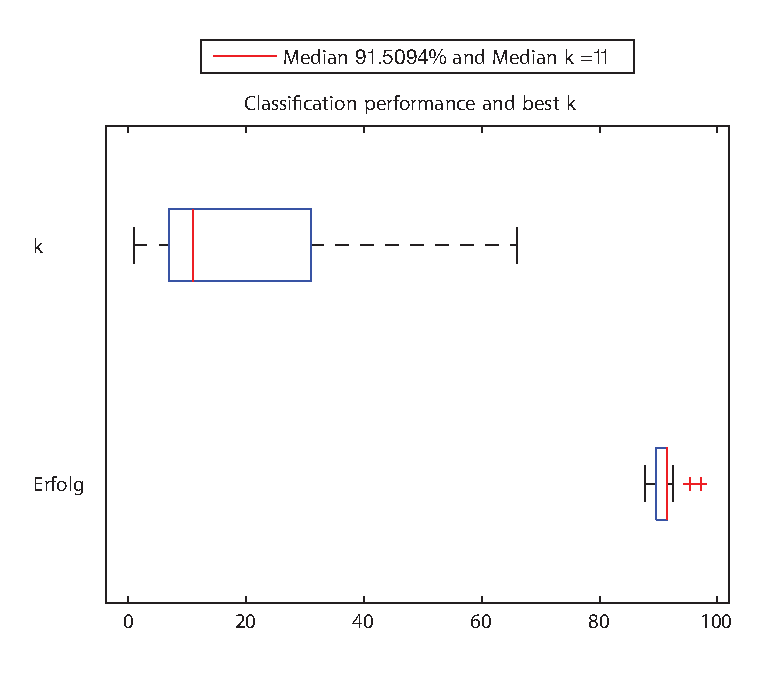
\includegraphics[width=9cm]{img/boxresults.eps}
		\caption{The upper Boxplot shows the derivation of the $k$ from the k-NN 
classifier. The Boxplot below shows the derivation of the classification performance}
		\label{fig:boxresults}
	\end{figure}

Figure~\ref{fig:bestresult} shows the best result of the k-NN classification 
with one of the test and training sets. But not all results are that good. 
Figure~\ref{fig:allresults} presents the performance of all 30 different test 
and training sets and their used $k$. Also the Median of the results is shown, 
which is $91,5094\%$ and the Median of the $k$ is $11$. But the median itself 
gives not a good representation of the derivation of the data. 
Figure~\ref{fig:boxresults} shows this information with boxplots.


\subsection{Evaluation of the Results}
\label{sec:kNNResults}

\begin{figure}
	\centering
	\setlength\figureheight{6cm} 
	\setlength\figurewidth{7cm}
	% This file was created by matlab2tikz v0.4.3.
% Copyright (c) 2008--2013, Nico Schlömer <nico.schloemer@gmail.com>
% All rights reserved.
% 
% The latest updates can be retrieved from
%   http://www.mathworks.com/matlabcentral/fileexchange/22022-matlab2tikz
% where you can also make suggestions and rate matlab2tikz.
% 
%
% defining custom colors
\definecolor{mycolor1}{rgb}{0,0,0.5625}%
%
\begin{tikzpicture}

\begin{axis}[%
width=\figurewidth,
height=\figureheight,
area legend,
scale only axis,
xmin=0.5,
xmax=3.5,
xtick={1,2,3},
xticklabels={1,11,21},
xlabel={k from k-NN},
ymin=0,
ymax=14,
ylabel={Median of classification error [\%]},
title={Lineplot of errors with k = 1  11  21}
]
\addplot[ybar,bar width=0.266666666666667\figurewidth,draw=black,fill=mycolor1] plot coordinates{(1,13.2075471698113)
(2,11.3207547169811)
(3,11.3207547169811)};

\addplot [
color=black,
solid,
forget plot
]
table[row sep=crcr]{
0.5 0\\
3.5 0\\
};
\end{axis}
\end{tikzpicture}%
	\caption{The median of the classification error rates of all 30 test sets for different values of $k$}
	\label{fig:ks}
\end{figure}

Our results show that the k-NN classifier is a powerful tool to classify the 
given data. But with a low value of $k$ the classification error enhances. Figure~\ref{fig:ks} shows the median of the classification error rates of all 30 test sets for different values of $k$. The smaller the error rate, the better the performance. Like we mentioned above the minimum is at a $k=11$.


\section{Wine Classification - Mahalanobis Distance}
\label{sec:Mahalanobis}

TODO


\subsection{Test and Training Set}
\label{sec:MahalanobisTestSet}

TODO


\subsection{Classification Performance}
\label{sec:MahalanobisPerformance}

TODO


\subsection{Comparison with k-NN}
\label{sec:MahalanobisComparison}

TODO


\section{Discriminant Functions for the Normal Density}
\label{sec:DiscriminantFunctions}

This section presents the computation of the discriminate function per hand and compares its results with the ones provided by MATLAB's classify function.


\subsection{Computation of the Discriminate Function per Hand}
\label{sec:Hand}

See Figure~\ref{fig:hws1} to Figure~\ref{fig:hws5}.
\begin{figure}
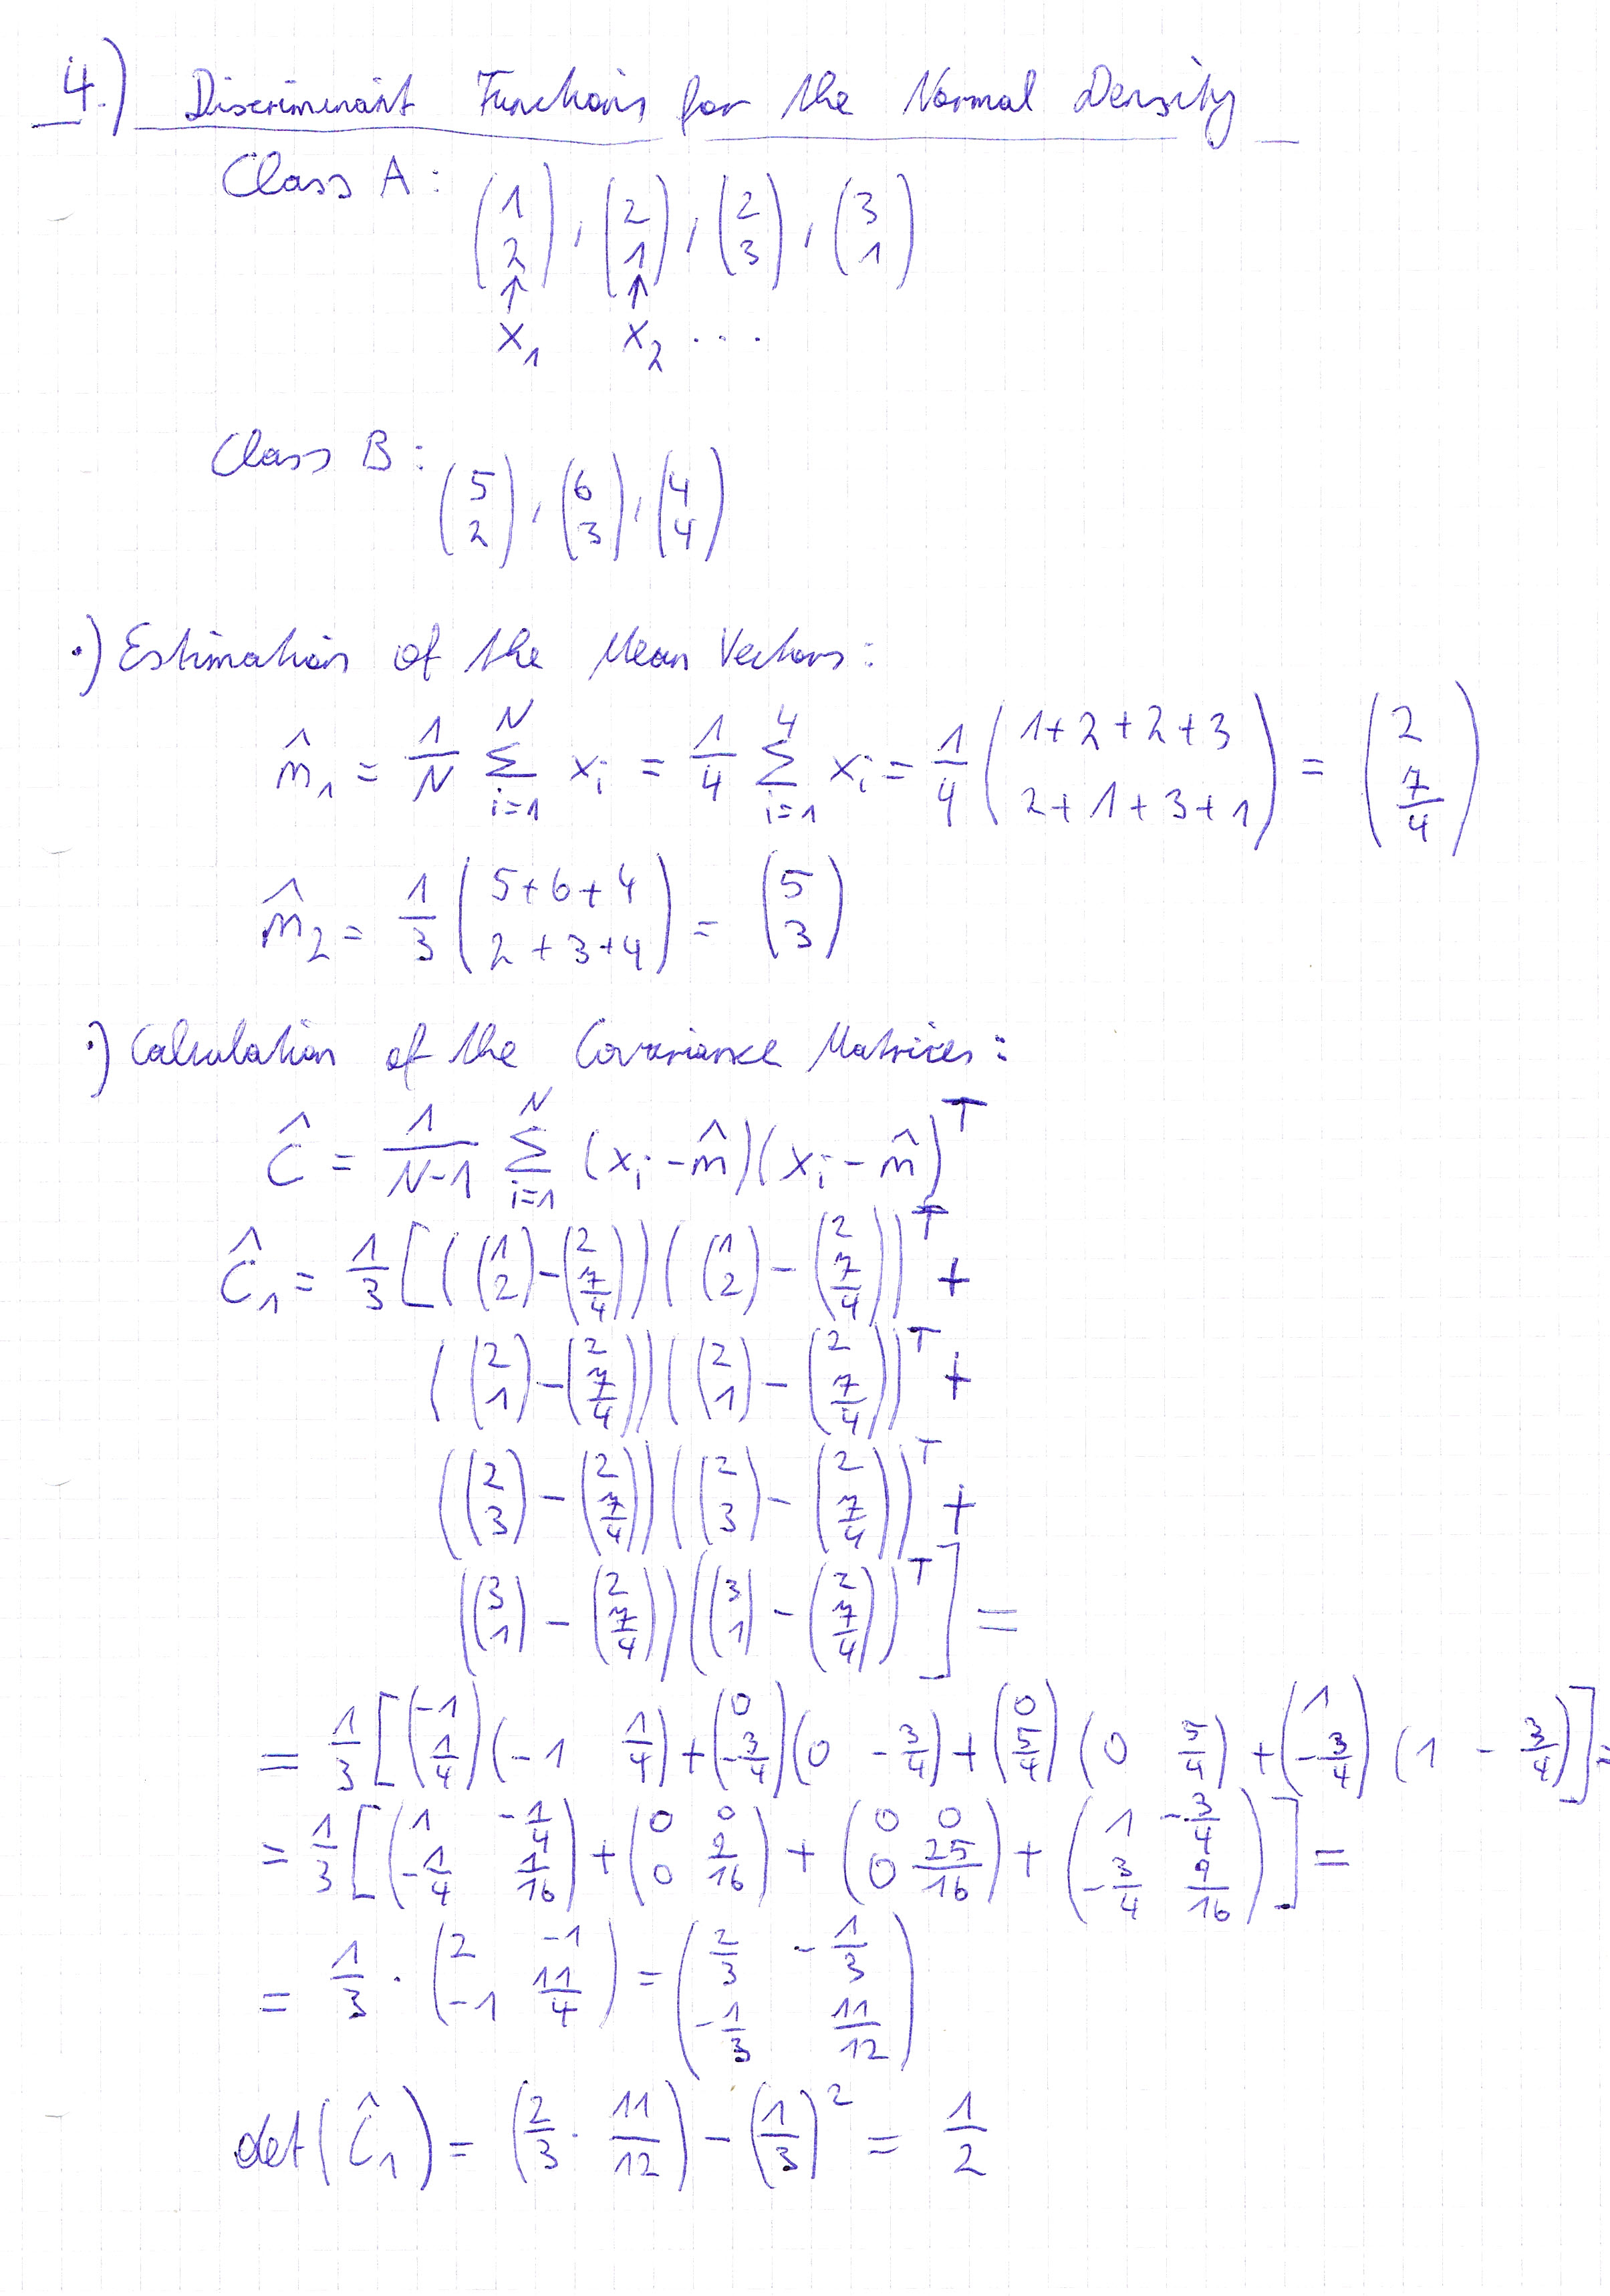
\includegraphics[width=14cm]{img/discriminantFunction1.jpg}
	\caption{Handwritten computation of the discriminate function, page 1}
	\label{fig:hws1}
\end{figure}

\begin{figure}
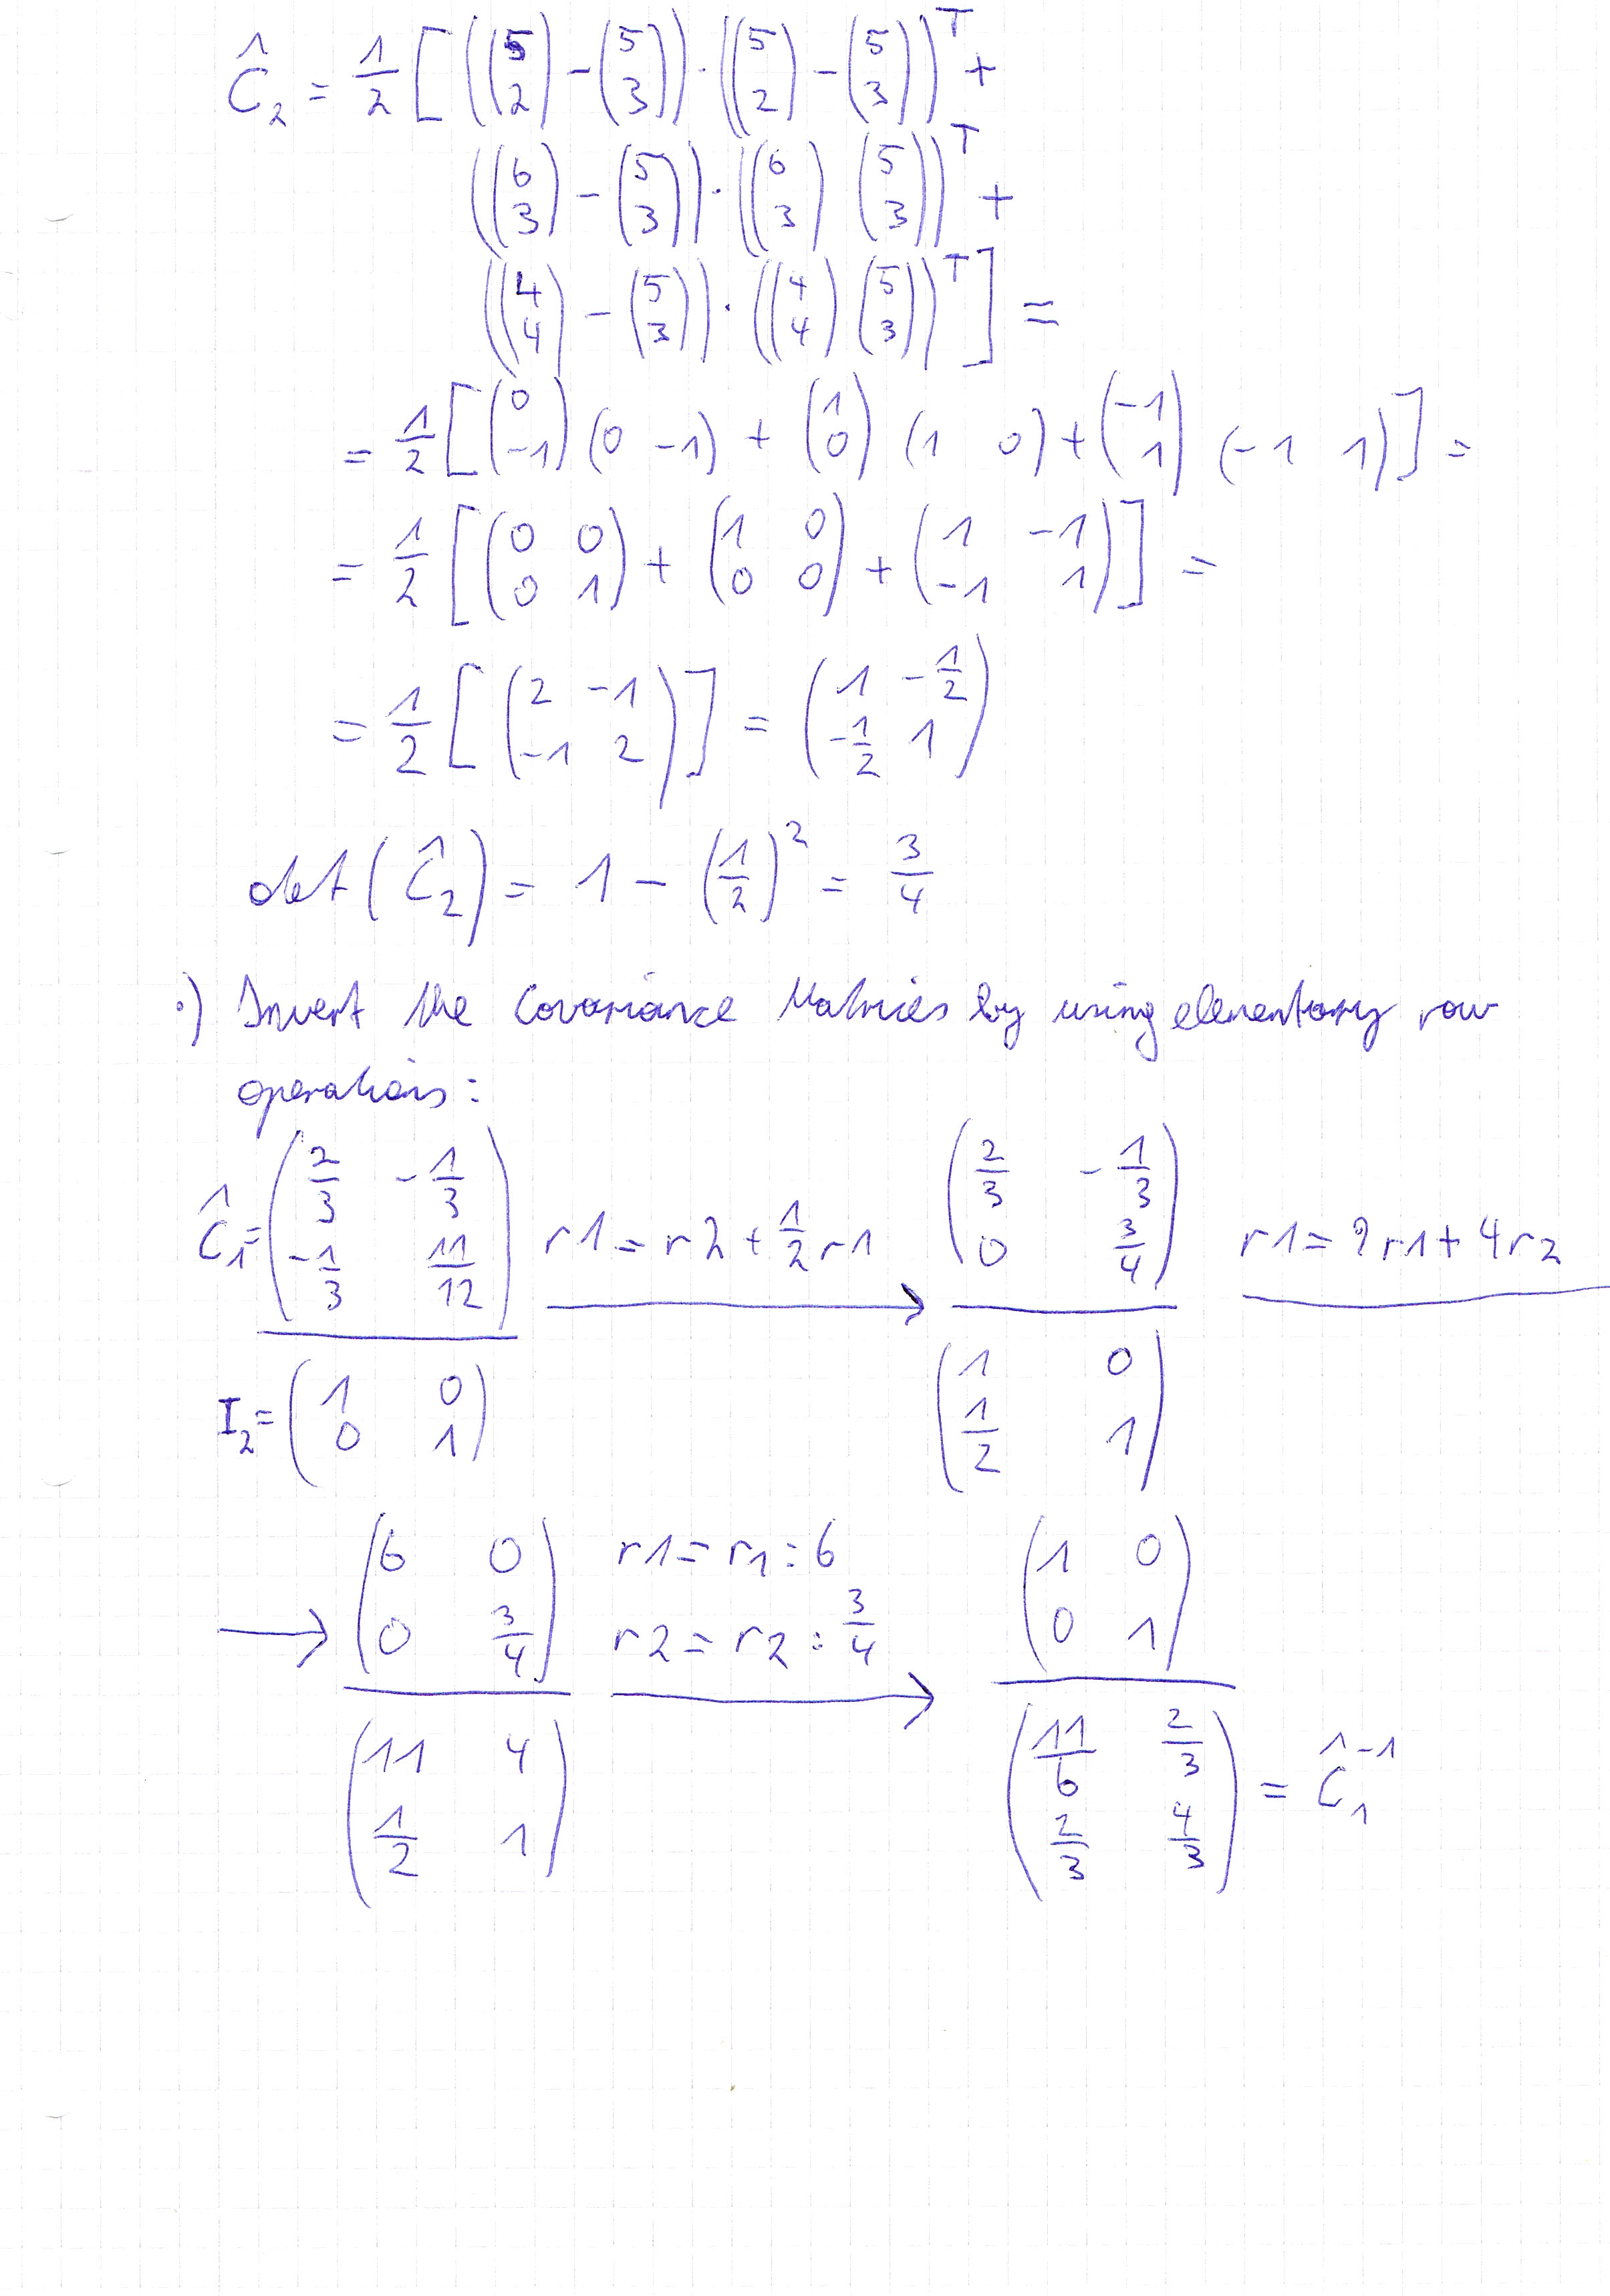
\includegraphics[width=14cm]{img/discriminantFunction2.jpg}
	\caption{Handwritten computation of the discriminate function, page 2}
	\label{fig:hws2}
\end{figure}

\begin{figure}
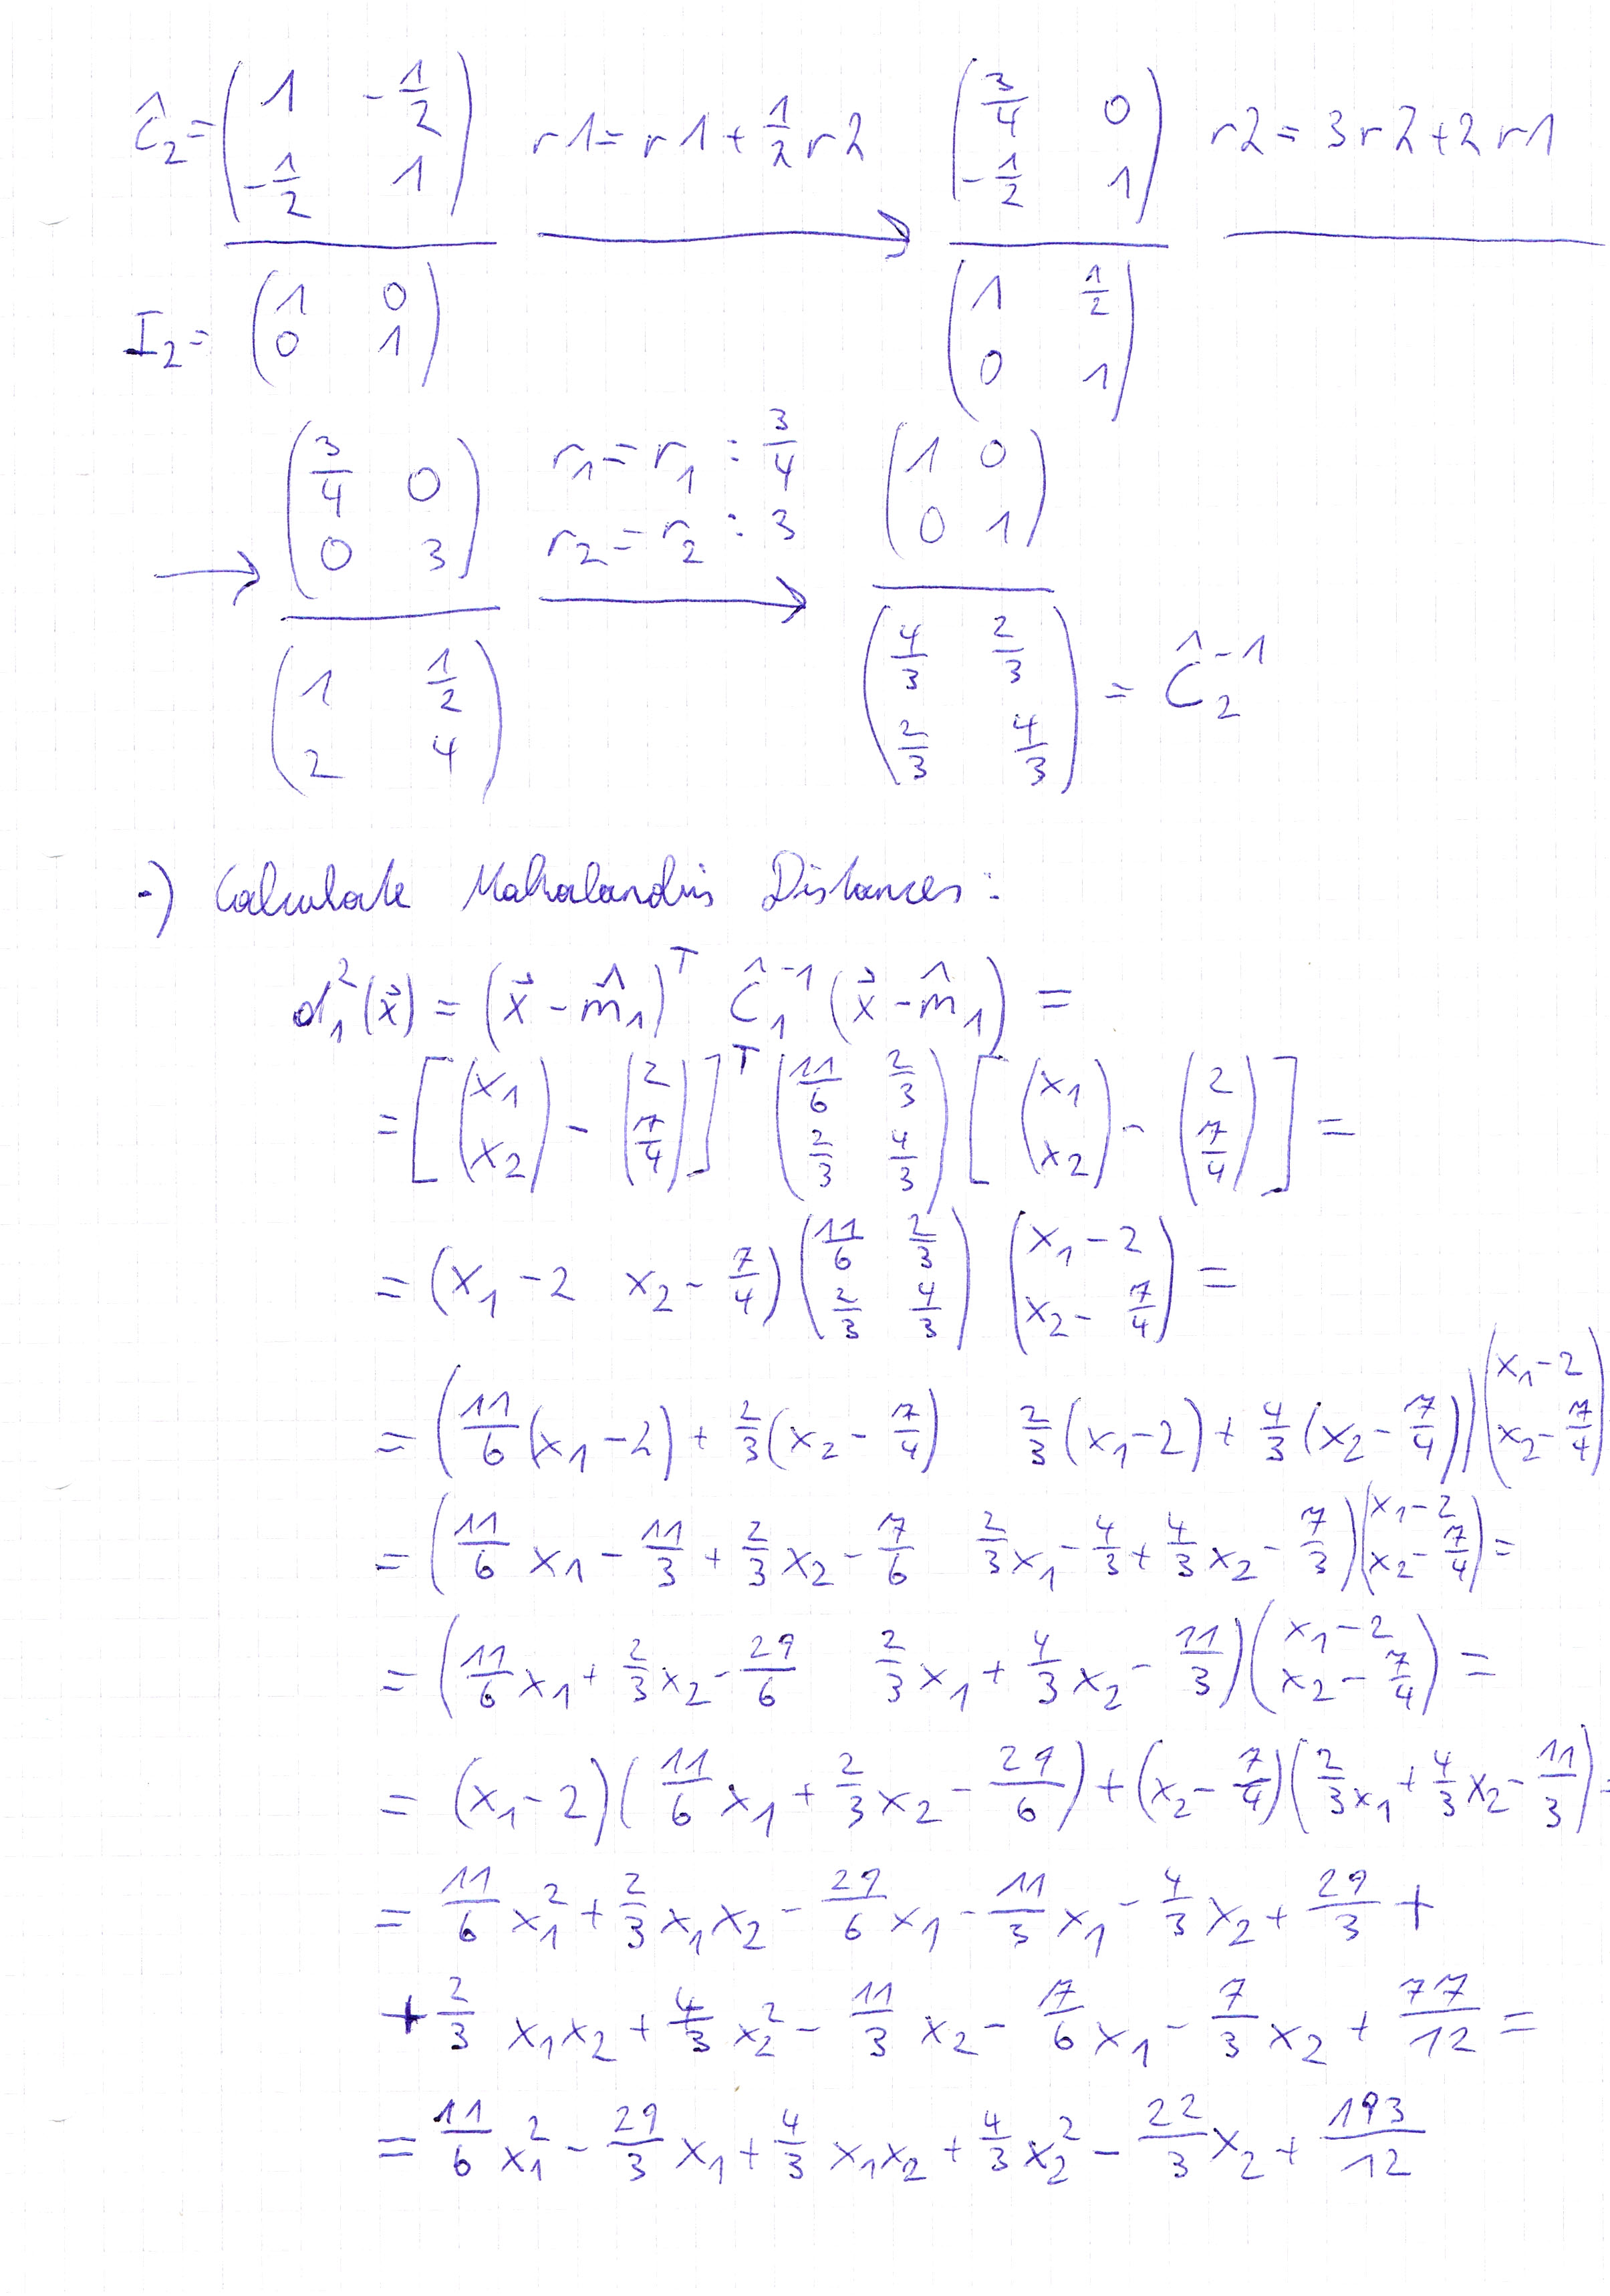
\includegraphics[width=14cm]{img/discriminantFunction3.jpg}
	\caption{Handwritten computation of the discriminate function, page 3}
	\label{fig:hws3}
\end{figure}

\begin{figure}
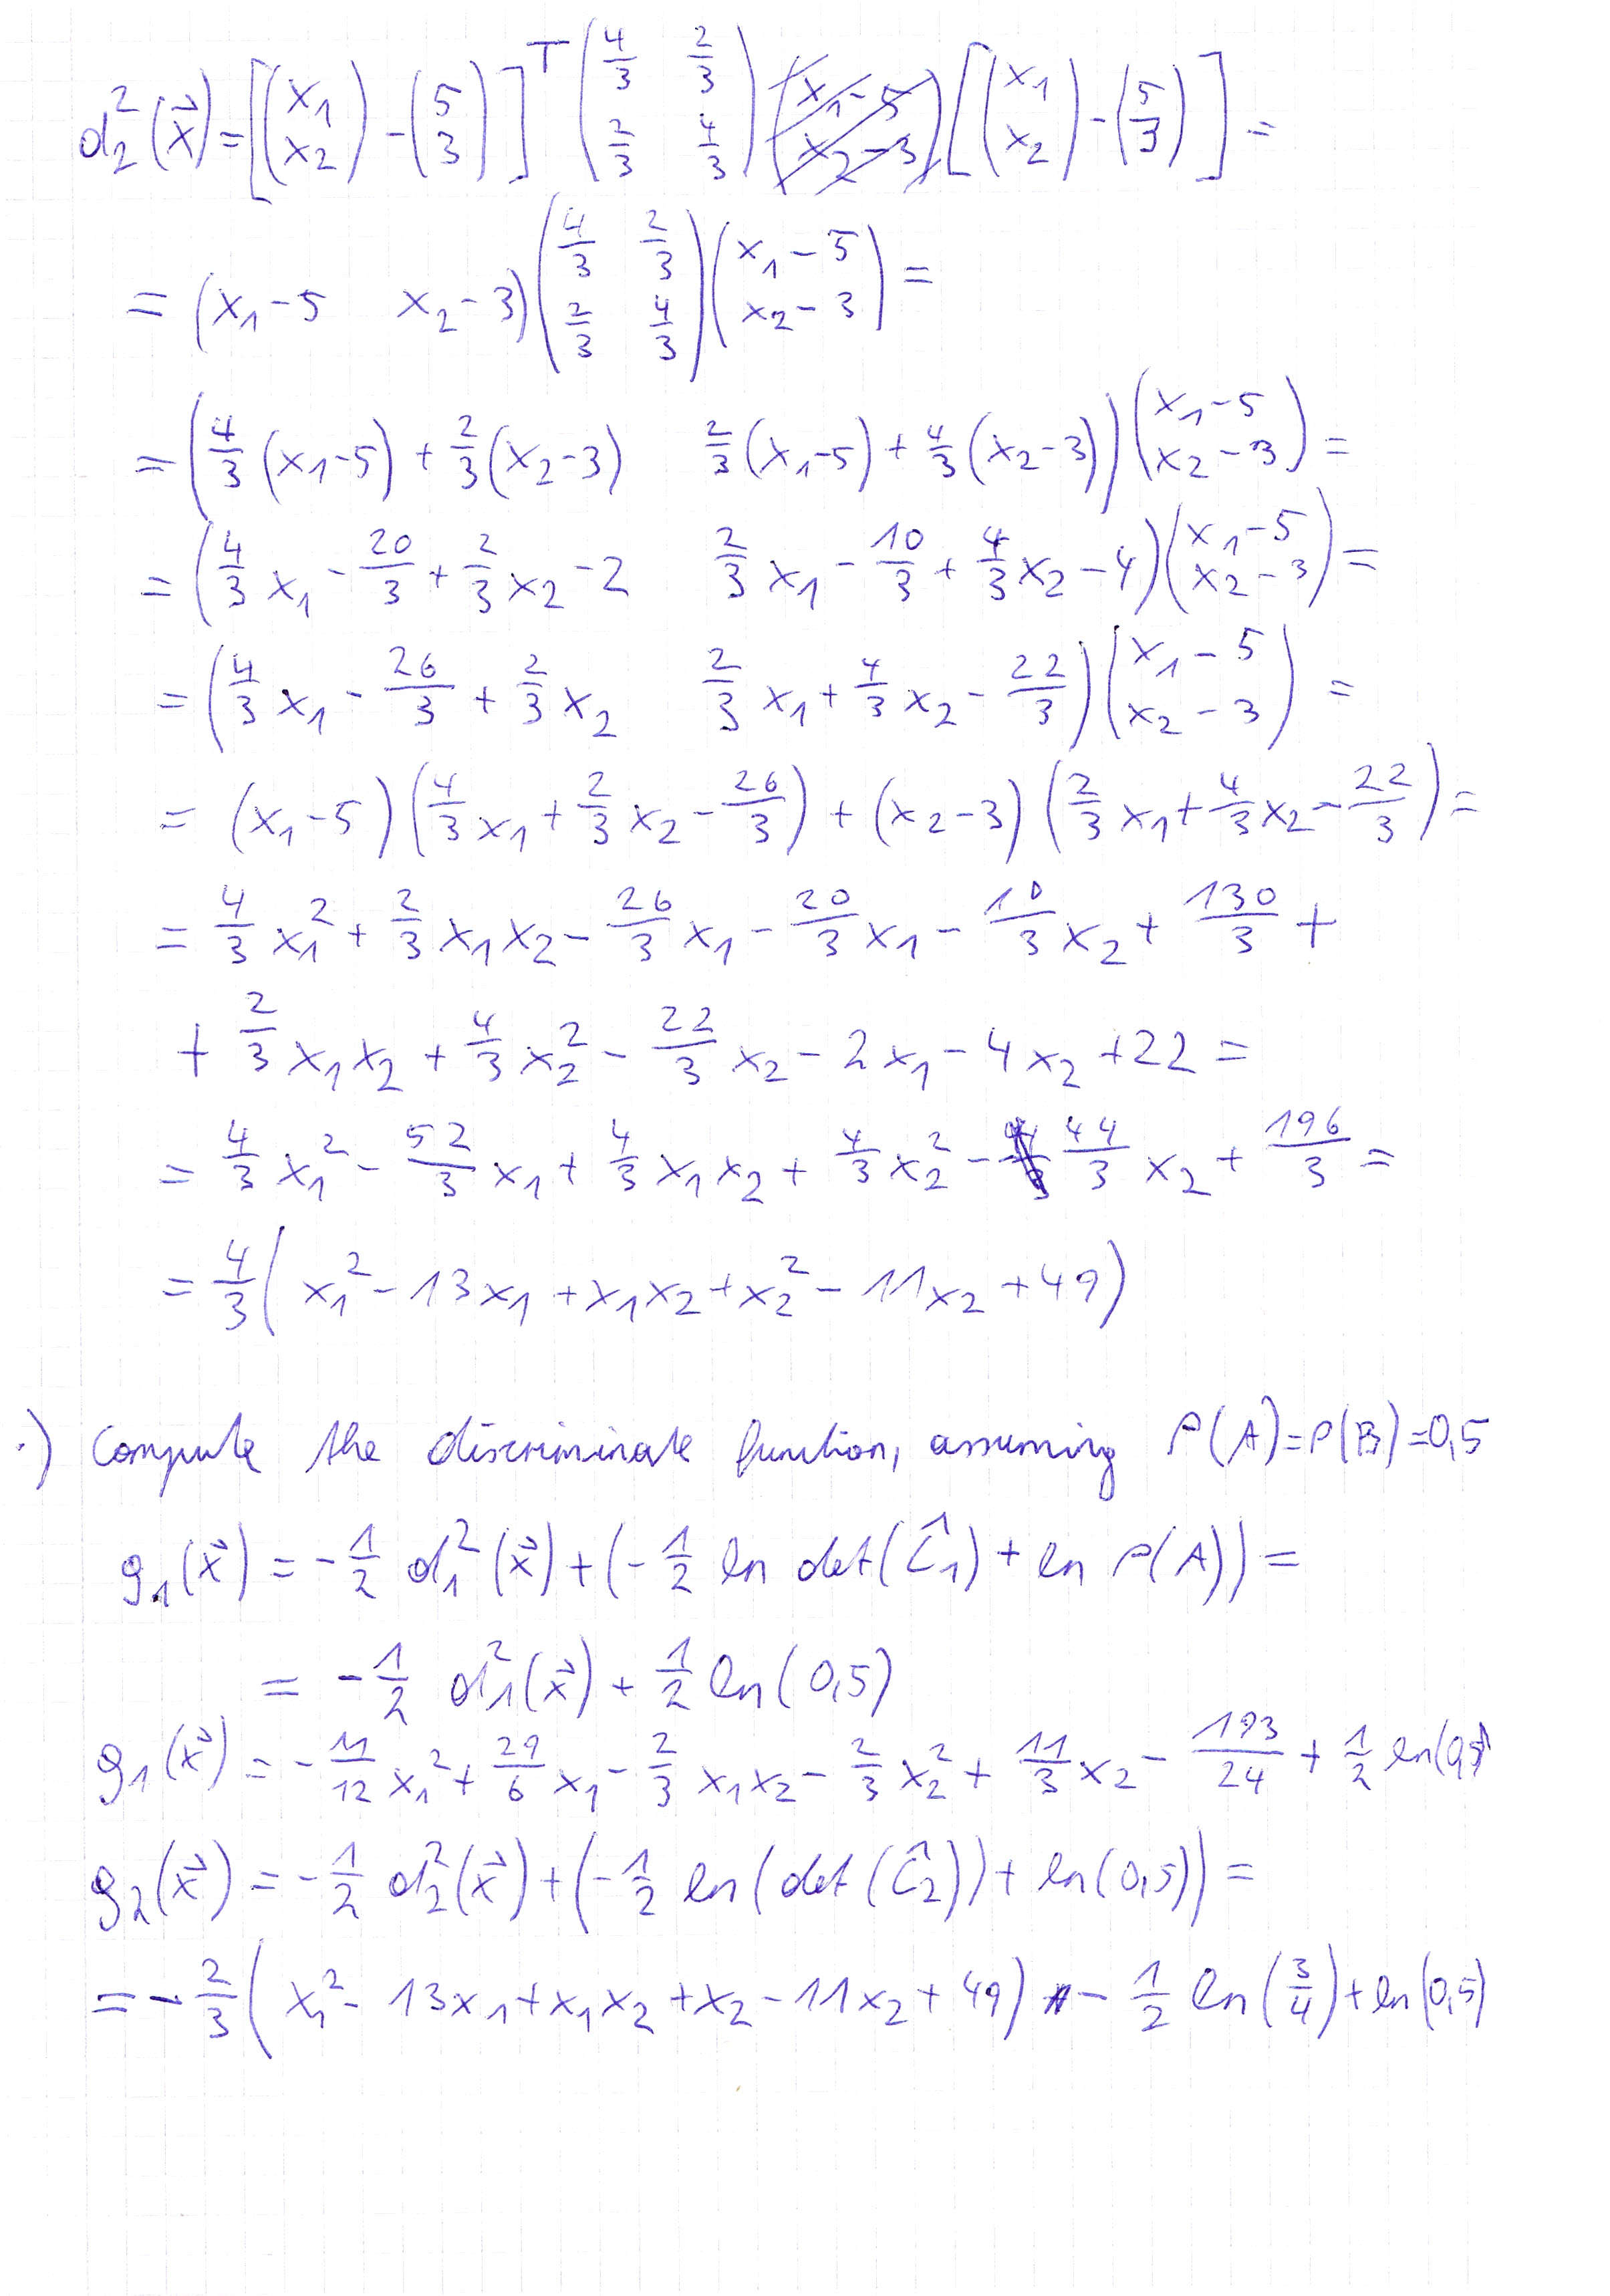
\includegraphics[width=14cm]{img/discriminantFunction4.jpg}
	\caption{Handwritten computation of the discriminate function, page 4}
	\label{fig:hws4}
\end{figure}

\begin{figure}
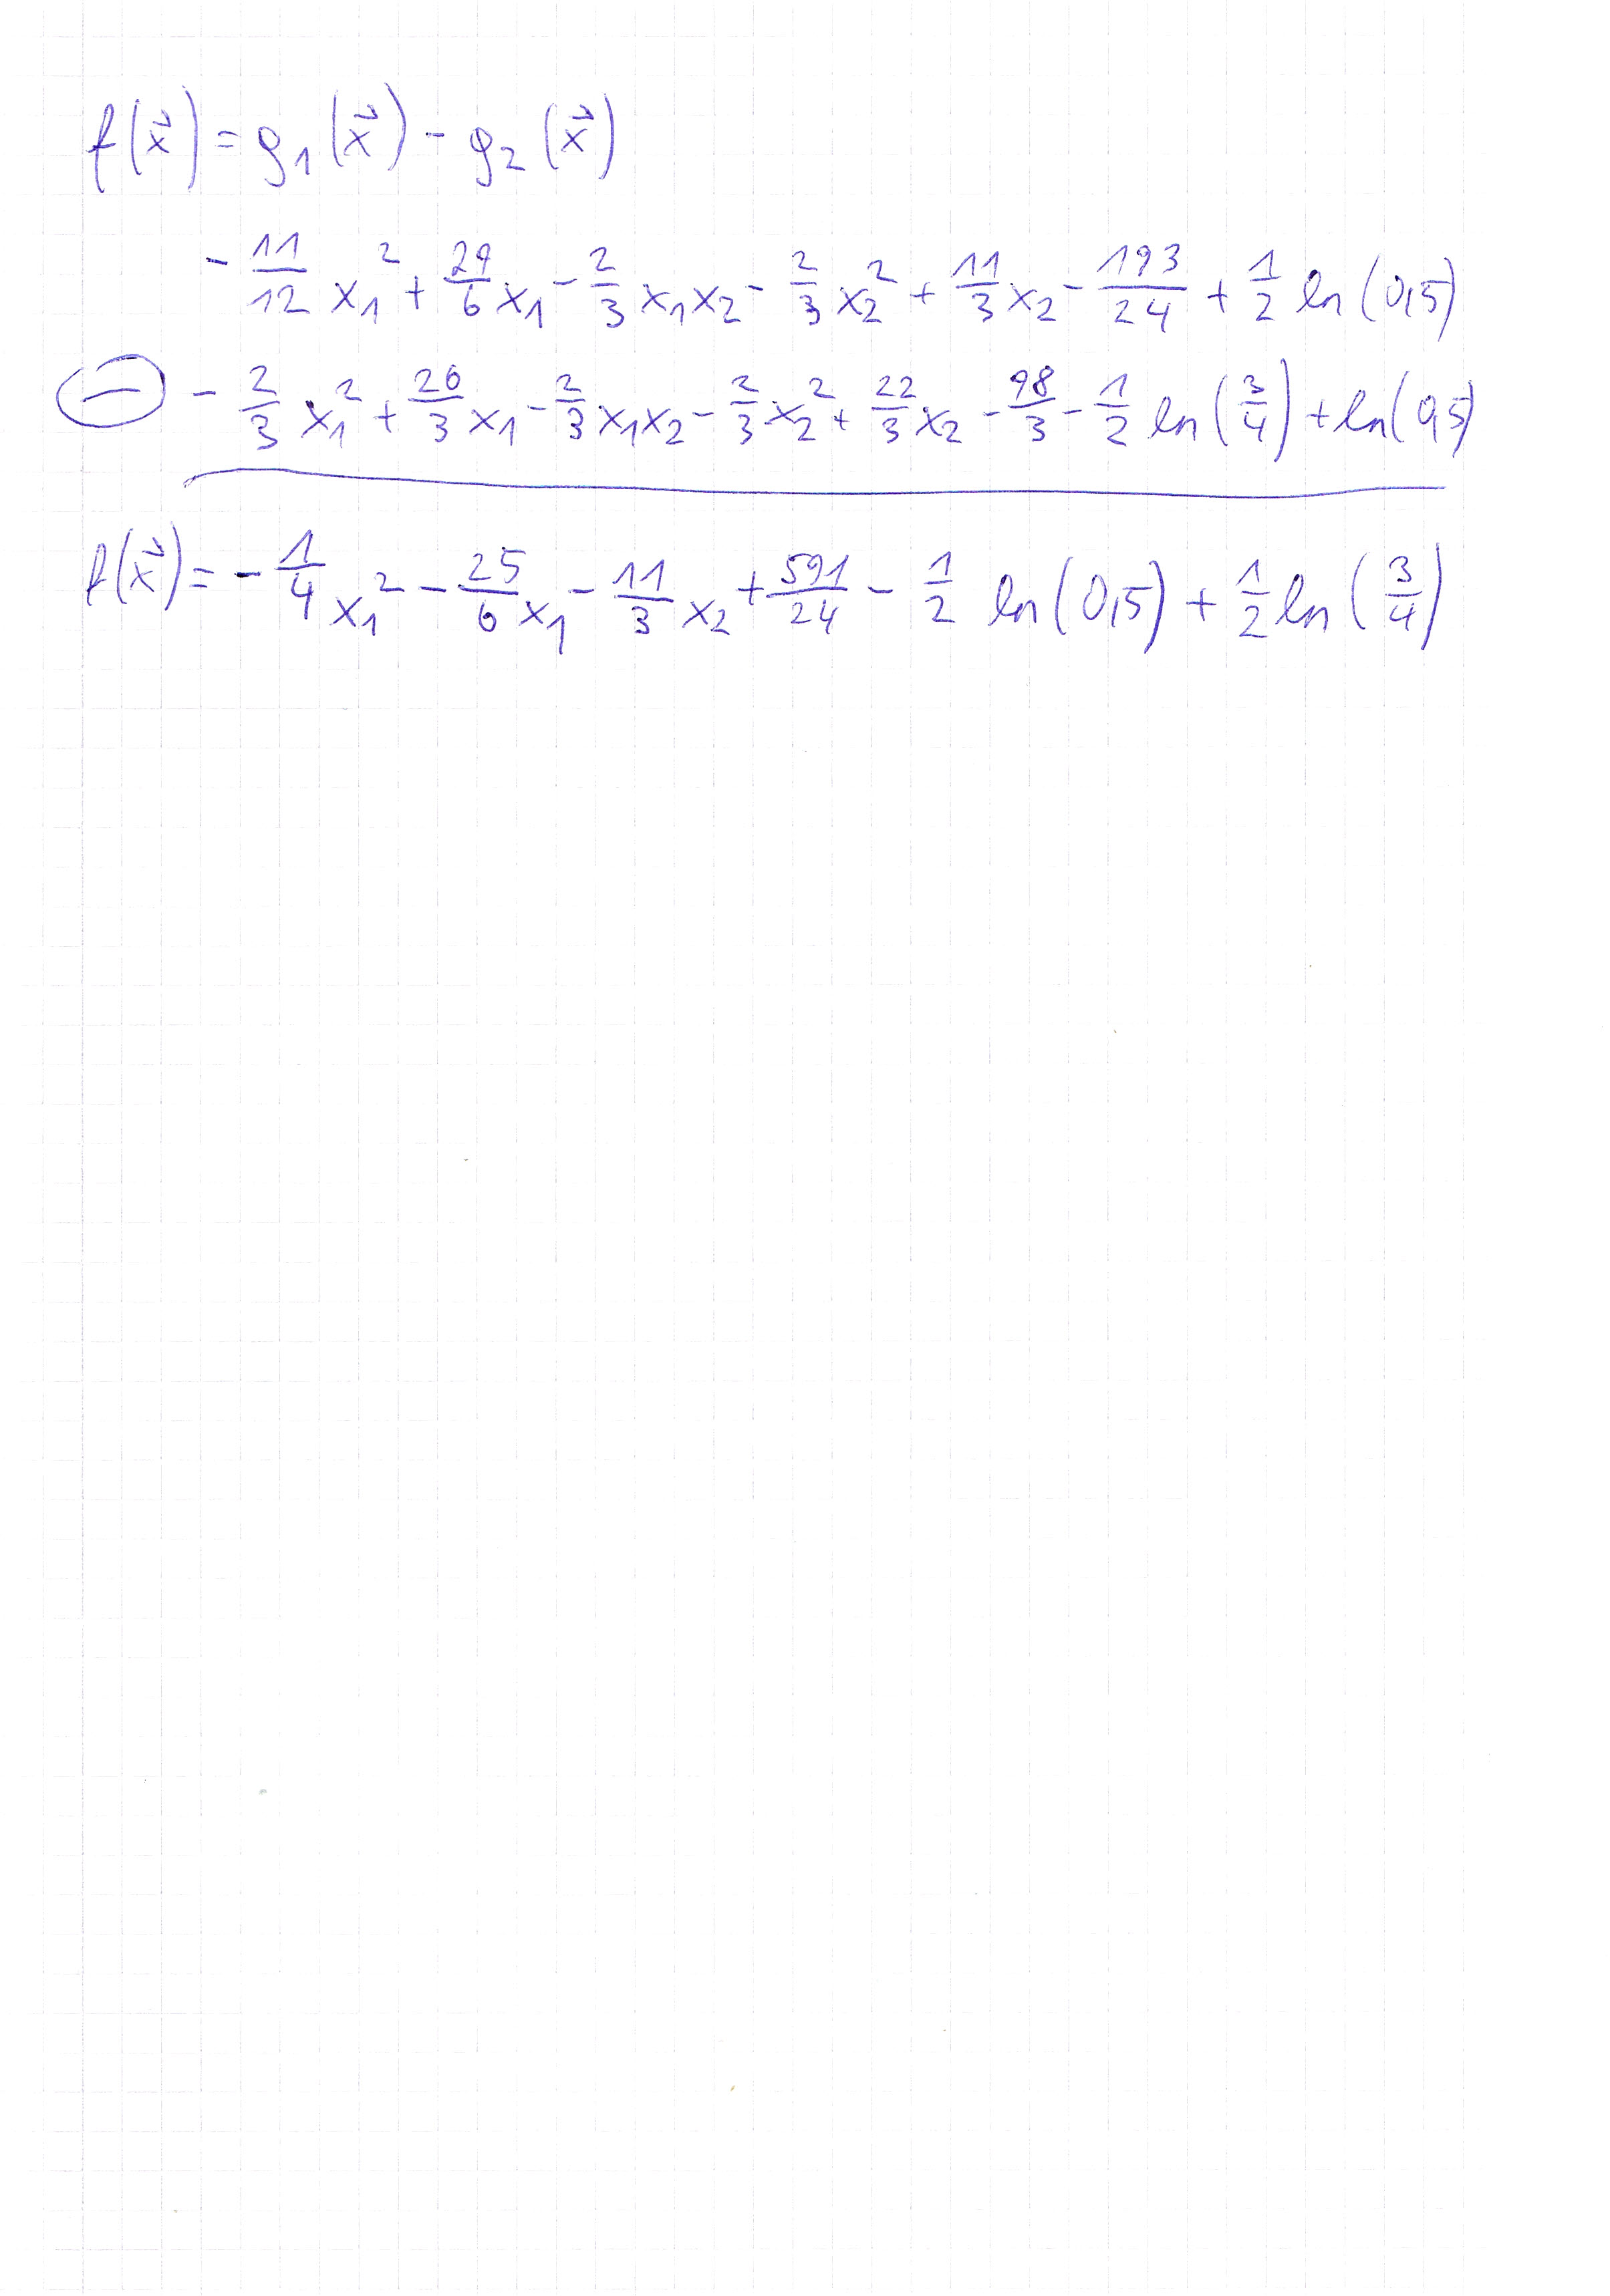
\includegraphics[width=14cm]{img/discriminantFunction5.jpg}
	\caption{Handwritten computation of the discriminate function, page 5}
	\label{fig:hws5}
\end{figure}

\subsection{Computation of the Discriminate Function in \texttt{MATLAB}}
\label{sec:Matlab}

As shown in  Figure~\ref{fig:disfunplot}, the handwritten computation of the discriminate function differs slightly from the one computed by MATLAB's classify function. It is also shown that the connection line between the mean values of the two classes is not perpendicular to the decision border. This is the case because the two classes' covariance matrices are different, and are not multiples of the identity matrix.

\begin{figure}
	\centering
        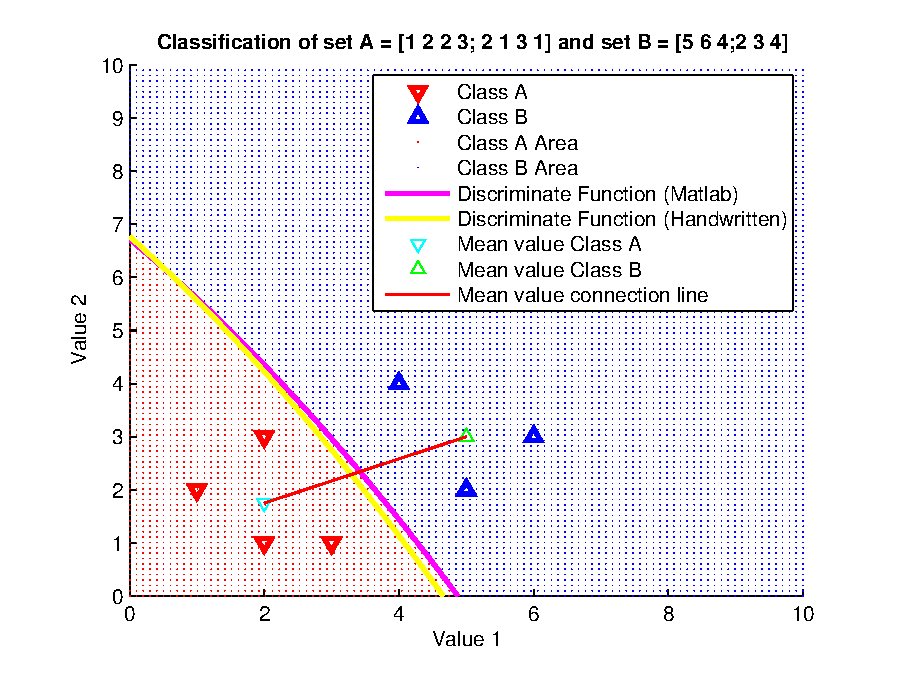
\includegraphics[width=14cm]{img/discriminantFunctionPlot.eps}
	\caption{The discriminate function, as computed by MATLAB's classify function (pink line).}
	\label{fig:disfunplot}
\end{figure}


\pagebreak
% Biblography


\fontsize{9}{10pt}
\bibliographystyle{plain}
\bibliography{literatur}

\end{document}

% vim:foldmethod=marker
